%\chapter{Nonlinear dynamics of two-dimensional lattices with complex structure}
\chapter{Нелинейная динамика двумерных решеток сложной структуры}

%\abstract*{The dynamics of two dimensional lattice structures is studied. The complexity of the structure includes non-neigboring interactions between the lattice masses, consideration of both translation and rotation interactions and also their  nonlinear character (physical nonlinearity). The asymptotic procedures are developed to obtain the governing nonlinear equations of motion in the continuum limit. The equations obtained are studied both analytically and numerically. Of special interest are the propagation and transverse instability of the plane solitary strain waves. It is shown that the dynamics of  longitudinal and shear waves is different in various two-dimensional lattices. The relationships for the elastic constants are obtained to characterize the type of the localized strain waves (tensile or compression), their transverse instability and possible auxetic behavior. Numerical solutions are obtained that describe unstable and stable dynamics of the plane longitudinal and shear waves.}

%The dynamics of two dimenesional lattice structures is studied. The complexity of the structure includes non-neigboring interactions between the lattice masses, consideration of both translation and rotation interactions and also their  nonlinear character (physical nonlinearity). The asymptotic procedures are developed to obtain the governing nonlinear equations of motion in the continuum limit. The equations obtained are studied both analytically and numerically. Of special interest are the propagation and transverse instability of the plane solitary strain waves. It is shown that the dynamics of  longitudinal and shear waves is different in various two-dimensional lattices. The relationships for the elastic constants are obtained to characterize the type of the localized strain waves (tensile or compression), their transverse instability and possible auxetic behavior. Numerical solutions are obtained that describe unstable and stable dynamics of the plane longitudinal and shear waves.

\fixme{Abstract оригинальной работы, заменить кратким описанием задачи, связать с основной работой каким-нибудь образом. В диссертации не выводятся модельные уравнения, а используются.}

В работе исследуется динамика механических структур с двумерной решеткой. Модель включает в себя взаимодействия между соседними и не соседними частицами решетки, учет как трансляционного, так и вращательного взаимодействий, а также их нелинейный характер (физическая нелинейность) взаимодействия. \fixme{Разработаны асимптотические процедуры для получения определяющих нелинейных уравнений движения в континуальном пределе}. Полученные уравнения исследуются как аналитически, так и численно. Особый интерес представляют распространение и поперечная неустойчивость плоских уединенных волн деформации. Показано, как отличается динамика продольных и поперечных волн разных двумерных решетках. Получены соотношения для упругих постоянных, характеризующие тип локализованных волн деформации (растяжение или сжатие), их поперечную неустойчивость и возможное ауксетическое поведение \fixme{$<-$ убрать}. Получены численные решения, описывающие неустойчивую и устойчивую динамику плоских продольных и поперечных волн.
	
\section{Введение}

\fixme{Перевод неточный, так как значительную часть нужно переделать}

%When dealing with the problem of description of materials with a complex microstucture, one usually wants to take into consideration either the influence of some specific dynamic processes on the stress-strain behaviour, or the influence of a complex microstructure, additional degrees of freedom or non-neigbouring interactions on the macro-parameters, and, in turn, on the model equations. 
При решении проблемы описания материалов со сложной микроструктурой обычно принимают во внимание или влияние некоторых конкретных динамических процессов на поведение напряженно-деформированного состояния, или влияние сложной микроструктуры, дополнительных степеней свободы, или наличие взаимодействия между несоседними элементами решетки на макропараметры системы и, в свою очередь, на уравнения модели.
	
%The modelling of the dynamical  behaviour of solid materials may be generally divided into two categories. Firstly, there are the discrete models, for which the equilibrium conditions, the kinematic conditions and the constitutive behaviour are formulated for each individual micro-structural element (cell) with respect to its neighbouring micro-structural elements \cite{Born,AskMetr, Askar, Ostoja}. Secondly, there are the continuum models, where the equilibrium conditions, the kinematic conditions and the constitutive behaviour are formulated for an assembly of micro-structural elements, using the continuum concepts of stress and strain, see, e.g., \cite{Maug,engbook97, erofeev}.
Моделирование динамического поведения твердых материалов можно разделить на две категории. Во-первых, это дискретные модели, для которых условия равновесия, кинематические условия и определяющее поведение сформулированы для каждого отдельного микроструктурного элемента (ячейки) по отношению к его соседним микроструктурным элементам \cite{Born, AskMetr, Askar, Ostoja}. Во-вторых, существуют континуальные модели, в которых условия равновесия, кинематические условия и определяющее поведение сформулированы для суперпозиции микроструктурных элементов с использованием континуальных концепций напряжения и деформации, см., Например, \cite{Maug, engbook97, erofeev}.
	
%A considerable advantage of discrete models in comparison to continuum models is that the inhomogeneous effects at the micro-level can be taken into account more accurately. The study of discrete models with non-neighboring interactions between the particles in the lattice has attracted considerable interest due to dispersion of the waves propagating in such a system \cite{AskMetr,Maug, Manev, Andrianov, Kosev, Mich, erem}. In particular, this is also important for the study of an influence of a microstructure of the materials. Dynamic processes in the one-dimensional lattices are investigated more extensively both in the linear and nonlinear consideration \cite{ Ostoja,Maug}, while two-dimensional lattices are mainly considered in the linearized case \cite{AskMetr, Ostoja, Tov}. Some two-dimensional processes may be modeled in the one-dimensional approximation, like plane waves propagation, while their transverse instability requires two-dimensional consideration.
Значительное преимущество дискретных моделей по сравнению с континуальными моделями состоит в том, что неоднородные эффекты на микроуровне могут быть учтены более точно. Изучение дискретных моделей с несоседними взаимодействиями между частицами в решетке вызвало значительный интерес из-за дисперсии волн, распространяющихся в такой системе \cite{AskMetr, Maug, Manev, Andrianov, Kosev, Mich, erem}. В частности, это также важно для изучения влияния микроструктуры материалов. Динамические процессы в одномерных решетках более широко исследуются как в линейном, так и в нелинейном рассмотрении \cite{Ostoja, Maug}, а двумерные решетки в основном рассматриваются в линеаризованном случае \cite{AskMetr, Ostoja, Tov}. Некоторые двумерные процессы можно моделировать в одномерном приближении, например распространение плоских волн, а их поперечная неустойчивость требует двумерного рассмотрения. 

%Considering everything mentioned above, it is obvious that discrete models can be utilized for the sake of accuracy. However, the number of representative micro-structural elements in a macro-structural configuration is normally very large, which causes the number of equations that has to be solved for a discrete system to become large as well. The discrete equations derived are very complex and stacked up, and cannot be solved analytically. So, the simplification and transition to some kind of a continuous model is needed in order to achieve a reasonable result for a further analysis.
Учитывая все вышесказанное, очевидно, что дискретные модели могут быть использованы как более точные. Однако количество репрезентативных микроструктурных элементов в макроструктурной конфигурации обычно очень велико, что приводит к тому, что количество уравнений, которые необходимо решить для дискретной системы, также становится огромным. Эта система, как правило, не может быть решена аналитически. Таким образом, континуальный переход от получаемых дискретных моделей к упрощенному виду является необходимым шагом для достижения разумных результатов для дальнейшего аналитического и численного анализа.
	
%In order to link the micro - and microscopic description, it is necessary to understand how exactly the transition from one description to another has to be made, and how to derive continuous equations from the discrete ones.
Чтобы связать микро- и микроскопическое описание моделей, необходимо понимать, как именно должен быть осуществлен переход от одного описания к другому и как вывести континуальные уравнения из дискретных.
	
%One of the famous methods is described in the works of \cite{AskMetr, SuiMetr}. In the linear case, both discrete and continuum equations may be considered analytically.  However, only a few discrete nonlinear equations, like the Toda lattice equation or the Ablowitz-Ladik equation, possess exact solutions \cite{Ablowitz}. That is why an approach based on a continuum limit of an original discrete equation is needed to obtain governing nonlinear continuum equations. The familiar acoustic branch continuum limit requires the long wavelength approximation and corresponds to the discrete model only for small wave numbers.
Один из известных методов описан в работах \cite{AskMetr, SuiMetr}. В линейном случае как дискретные, так и континуальные уравнения можно рассматривать аналитически. Однако только несколько дискретных нелинейных уравнений, таких как уравнение цепочки Тода или уравнение Абловица-Ладика, имеют точные решения \cite {Ablowitz}. Вот почему для получения определяющих нелинейных уравнений сплошной среды необходим подход, основанный на континуальном пределе исходного дискретного уравнения. Известный континуальный предел акустической ветви требует длинноволнового приближения и соответствует дискретной модели только для малых волновых чисел.
	
%A well-known enhanced continuum formulation is the Cosserat continuum (or micro-polar continuum), which is an augmentation of the standard Boltzmann continuum by three rotational degrees of freedom. The rotational degrees of freedom introduce a "bending effect" in the constitutive formulations, and the characteristic length scale is therefore governed by the ratio between this additional bending stiffness and the normal stiffness. The development of the Cosserat continuum formulation started at the beginning of this century with the concept of the inclusion of rotational degrees of freedom was introduced for the first time.
\fixme{Хорошо известной усовершенствованной формулировкой континуума является континуум Коссера (или микрополярный континуум), который является дополнением стандартного континуума Больцмана тремя вращательными степенями свободы. Вращательные степени свободы создают «эффект изгиба» в составах компонентов, и поэтому характерный масштаб длины определяется соотношением между этой дополнительной жесткостью на изгиб и нормальной жесткостью. Разработка континуума Коссера началась в начале этого века, когда впервые была введена концепция включения вращательных степеней свободы.}
	
%The problem of reasonable simplification when describing properties of materials is closely connected with the question of what can be neglected and what must be included. This can be resolved by utilizing a range of asymptotic methods. This is particularly important when dealing with nonlinear processes in crystal lattices. \cite{Maug,Zabus, engbook83, Manev, Zab, engber, PorBer, PorBer2, porkros, porosmich1, porosmich2}
Проблема выбора корректных упрощений при описании свойств материалов тесно связана с вопросом о том, чем можно пренебречь, а чем нельзя. Эту проблему можно решить, используя ряд асимптотических методов. Это особенно важно при рассмотрении нелинейных процессов в кристаллических решетках \cite{Maug, Zabus, engbook83, Manev, Zab, engber, PorBer, PorBer2, porkros, porosmich1, porosmich2}.
	
%Each of the approaches mentioned above have led to significant advances connected with higher precision of materials with microstructure description: from breathers and solitary waves to discovery of auxetic properties of 2D crystals \cite{erof_pav}.
Каждый из упомянутых выше подходов привел к значительному прогрессу в этом разделе механики, связанному с повышением точности описания процессов микроструктуры материалов: от бризеров и уединенных волн до открытия ауксетических свойств двумерных кристаллов \cite{erof_pav}.
	
%In the following sections authors show the asymptotic simplification procedure developed to make nonlinear analysis feasible.
\fixme{В следующих разделах авторы показывают процедуру асимптотического упрощения, разработанную для обеспечения возможности нелинейного анализа.}
%Later, it is applied to obtain Kadomtsev-Petviashvili\cite{kadpet} type equations and their solutions for the cases of generalized square and graphene lattices. Finally, it helps to describe the system's behaviour in terms of stability and later utilize the findings in the numerical simulation.
Далее он применяется для получения уравнений типа Кадомцева-Петвиашвили \cite {kadpet} и их решений для случаев обобщенных квадратных и графеновых решеток. Наконец, это помогает описать поведение системы с точки зрения устойчивости, а затем использовать результаты \textbf{численного моделирования}.
	
%\section{Two-dimensional waves in a generalized square lattice}
\section{Двумерные волны в обобщенной квадратной решетке}
	
%\subsection{Statement of the problem}
\subsection{Постановка задачи}
	
%A generalized two-dimensional square lattice model  considers  additional long-range interactions of the central particle with mass $M$, see \cite{porkros} for details. The model includes quadratic and cubic nonlinearity in the elastic inter-particle forces in addition to the conventional Hookean interaction.
Обобщенная двумерная модель квадратной решетки рассматривает дополнительные дальнодействующие взаимодействия центральной частицы с массой $M$ \cite{porkros}. Модель включает квадратичную и кубическую нелинейность упругих межчастичных сил в дополнение к обычному гуковскому взаимодействию.
%The central particle with the number ${m,n}$ interacts with four horizontal and vertical neighbors by the springs with linear rigidity $C_1$ and non-linear rigidities $Q$ and $Q_3$. The relative distance in the unstrained state is assumed to be equal to $l$. 
Центральная частица с номером ${m, n}$ взаимодействует с четырьмя горизонтальными и вертикальными соседями посредством пружин с линейной жесткостью $C_1$ и нелинейной жесткостью $Q$ и $Q_3$. Относительное расстояние в ненапряженном состоянии принимается равным $l$. \fixme{Добавить рисунок.}
%Then the total potential energy is
Тогда полная потенциальная энергия суть
\[
\Pi=~\Pi_1+\Pi_2+\Pi_3.
\]
%where $\Pi_1$ accounts for interactions with nearest four particles in the horizontal and vertical directions,
где $\Pi_1 $ учитывает взаимодействия с ближайшими четырьмя частицами в горизонтальном и вертикальном направлениях,
\[
\Pi_1~=~\frac{1}{2} C_1 \sum_{i=1}^{4}\triangle l_i^2+\frac{1}{3} Q~ \sum_{i=1}^{4}\triangle l_i^3+\frac{1}{4} Q_3~ \sum_{i=1}^{4}\triangle l_i^4,
\]
%where $x_{m,n}$, $y_{m,n}$ are the horizontal and vertical displacements of particle $m,n$. The expressions for elongations of the springs, $\triangle l_i$ are  \cite{porkros}
где $x_{m, n}$, $y_{m, n} $ --- горизонтальное и вертикальное смещения частицы $m, n$. Выражения для удлинения пружин $\triangle l_i$ следующие: \cite {porkros}
\[
\triangle l_1~=~x_{m+1,n}-x_{m,n},~ \triangle l_2~=~y_{m,n+1}-y_{m,n},~\triangle l_3~=~x_{m,n}-x_{m-1,n},~ \triangle l_4~=~y_{m,n}-y_{m,n-1}
\]
%where the springs are numbered counter-clockwise. Next group of interacting particles is composed by four diagonal neighboring particles  whose positions are described by the angles $\phi~=~\pi/4+ \pi~k/2, ~k=0,...,3$. The linear rigidity of the connecting springs is $C_2$ while the nonlinear rigidities are $P$ and $P_3$. The contribution to the potential energy is
где пружины пронумерованы против часовой стрелки. Следующая группа взаимодействующих частиц состоит из четырех диагональных соседних частиц, положение которых описывается углами $\phi~=~\pi/4+ \pi~k/2, ~k=0,...,3$. Линейная жесткость соединительных пружин равна $C_2$, а нелинейная жесткость --- $P$ и $P_3$. Вклад в потенциальную энергию равен
\[
\Pi_2~=~\frac{1}{2} C_2 \sum_{i=5}^{8}\triangle l_i^2+\frac{2\sqrt{2}}{3} P~ \sum_{i=5}^{8}\triangle l_i^3+ P_3~ \sum_{i=5}^{8}\triangle l_i^4,
\]
%The expressions for elongations may be found in \cite{porkros}.
Выражения для удлинений можно найти в \cite {porkros}.

%The final group consists of eight  long -range  particles whose positions are characterized by the angels  $\psi$, $\theta$, so as $\tan \psi=1/2$, $\tan \theta=2$, see figure in  \cite{porkros}. Then the contribution to the energy is
Последняя группа состоит из восьми дальнодействующих частиц, положения которых характеризуются ангелами $\psi$, $\theta$, так что $\tan \psi = 1/2$, $\tan \theta=2$, см. рисунок из \cite{porkros}. \fixme{Добавить рисунок}. Тогда вклад в энергию равен
$$
\Pi_3~=~\frac{1}{2} C_3 \sum_{i=9}^{16}\triangle l_i^2+\frac{5\sqrt{5}}{3} S \sum_{i=9}^{16}\triangle l_i^3+\frac{25}{4} S_3 \sum_{i=9}^{16}\triangle l_i^4,
$$
%where $C_3$ is linear rigidity, $S$ and $S_3$ are nonlinear rigidities. The expressions for elongations may be found in \cite{porkros}.
где $C_3$ - линейная жесткость, $S$ и $S_3$ - нелинейные жесткости.

%The kinetic energy is
Кинетическая энергия выражается следующим образом,
\[
T~=~\frac{1}{2} M\left(\dot{x}_{m,n}^2+\dot{y}_{m,n}^2\right).
\]

%Then the Lagrangian, $L=T-\Pi$, may be composed, and the Hamilton-Ostrogradsky variational principle is applied to obtain the discrete governing equations of motion, see   \cite{porkros} for details.
Таким образом, можно составить лагранжиан $L = T- \Pi$ и применить вариационный принцип Гамильтона-Остроградского для получения уравнений движения дискретной модели, подробности см. в \cite{porkros}.

\fixme{При дальнейшем выводе лучше ссылаться сразу на две работы --- главу из книги и статью.}

\subsection{Auxetic behavior in the linearized model}
For small wave numbers, one assumes that  the continuum displacements of the central particle $x_{m,n}$, $y_{m,n}$ are  $u(x, y, t)$, $v(x, y, t)$ thus introducing predominantly longitudinal waves propagation. Then the  Taylor series for the  neighboring particles are
\[
x_{m\pm1,n\pm1}~=~ ~u\pm l~ u_x\pm  l~ u_y+\frac{1}{2} l^2 u_{xx}+  l^2 u_{xy}+\frac{1}{2} l^2 u_{yy}+...
\]
Then the two-dimensional linearized continuum equations are
\[
M~u_{tt}-\frac{l^2}{5}\left(\frac{}{} 5(C1+C_2)+34 C_3 \frac{}{}\right)~u_{xx}-\frac{2l^2}{5}\left(\frac{}{}5C_2+16 C_3\frac{}{}\right) v_{xy}-
\]
\begin{equation}
	\frac{l^2}{5}\left(\frac{}{}5C_2+16 C_3\frac{}{}\right) u_{yy}~=~0,
	\label{aux1}
\end{equation}

\[
M~v_{tt}-\frac{l^2}{5}\left(\frac{}{}5(C1+C_2)+34 C_3\frac{}{}\right)~v_{yy}-\frac{2l^2}{5}\left(\frac{}{}5C_2+16 C_3\frac{}{}\right)u_{xy}-
\]
\begin{equation}
	\frac{l^2}{5}\left(\frac{}{}5C_2+16 C_3\frac{}{}\right) v_{xx}~=~0.
	\label{aux2}
\end{equation}

Equations (\ref{aux1}), (\ref{aux2}) are related to the equations of motion of the cubic crystals provided that the elastic cubic constants $C_{11}$, $C_{12}$ and $C_{44}$ are connected with our constants $C_1$, $C_2$ and $C_3$ as

\[
C_{11}~=~\frac{1}{5l}\left(5(C_1+C_2)+34 C_3\right),~ C_{44}~=~\frac{1}{5l}\left(5C_2+16 C_3\right),
\]
\begin{equation}
	C_{12}+C_{44}~=~\frac{2}{5 l}\left( 5 C_2+16 C_3\right). \label{relmod}
\end{equation}
These relationships hold only if $C_{12}=C_{44}$ or for the Cauchy condition  for materials with cubic symmetry when only central interactions are taken into account \cite{Born}. However, they fail, e.g., for cubic metals \cite{thomas_cauchy}.

The relationships for the Poisson ratios for cubic crystals can be found in Ref. \cite{erof_pav}. For the case $C_{12}=C_{44}$ they are
\[
\nu_{<100,001>}~=~\frac{C_{12}}{C_{11}+C_{12}},~\nu_{<111,001>}~=~\frac{4 C_{12}^2}{2C_{12}(C_{11}-C_{12})+C_{11}(C_{11}+C_{12})},
\]
\[
\nu_{<110,110>}~=~\frac{(C_{11}+C_{12})(C_{11}-2 C_{12})}{(C_{11}-C_{12})(C_{11}+2C_{12})+2C_{11} C_{12}},\nu_{<111,111>}~=~\frac{C_{11}}{2(C_{11}+3C_{12})}.
\]
Using Eqs. (\ref{relmod}) one obtains
\[
C_{11}-C_{12}=\frac{l^2}{5 M}\left( 5C_1+18 C_3\right), ~C_{11}-2C_{12}~=~\frac{l^2}{5M}\left(C_1 - C_2 + 2 C_3\right).
\]
Only the last expression can be negative giving rise to a negative value of $\nu_{<110,110>}$. One can see that the long- range interaction described by the coefficient $C_3$, adds positiveness in the relation $C_1 - C_2 + 2 C_3$.


%\subsection{Continuum nonlinear equations}
\subsection{Нелинейные уравнения континуальной модели}
\fixme{Это по идее будет нужно}
%The  equations of motion  obtained from the variational principle are further reduced when the plane waves propagating in horizontal direction are studied   \cite{porkros}. For simplicity let us consider  nonlinear  waves propagating in a horizontal direction along the  $x$ axis and weakly perturbed in the transverse direction along the  $y$ axis. The transverse weakness is characterized by the small parameter $\varepsilon~\ll~1$, the continuum displacements are assumed to be the functions of slow transverse variable $Y~=~\varepsilon y$. The same small parameter is used to account for the weakly nonlinear waves, however, its utilization depends on whether transverse variations of  longitudinal or shear waves are studied.
Уравнения движения, полученные из вариационного принципа, дополнительно сокращаются при изучении плоских волн, распространяющихся в горизонтальном направлении \cite {porkros}. Для простоты рассмотрим нелинейные волны, распространяющиеся в горизонтальном направлении вдоль оси $ x $ и слабо возмущенные в поперечном направлении вдоль оси $y$. Поперечная слабость характеризуется малым параметром $\varepsilon ~ \ll ~ 1$, смещения континуума считаются функциями медленной поперечной переменной $Y ~=~ \varepsilon y$. Тот же самый малый параметр используется для учета слабонелинейных волн, однако его использование зависит от того, исследуются ли поперечные вариации продольных или поперечных волн. 

\subsubsection{Продольные волны}
\fixme{Тоже нужно, но не в качестве subsection}

%For small wave numbers, one assumes that  the continuum displacements of the central particle $x_{m,n}$, $y_{m,n}$ are  $u(x, Y, t)$, $v(x, Y, t)$. Of special interest are the localized waves keeping their shape and velocity on propagation. These waves exist under the balance between nonlinearity and dispersion. Dispersion terms are the higher-order linear derivative terms arising from the Taylor expansion. Their smallness may be provided by choosing $l~=~\varepsilon~ h$. Nonlinear terms turn out of the same order under an assumption about smallness of the continuum displacement of the form $\varepsilon^2~u(x, Y, t)$, $\varepsilon^3~v(x, Y, t)$, also the nonlinear rigidities should be $P=P/\varepsilon$, $Q=Q/\varepsilon$, $S=S/\varepsilon$,  and cubic nonlinear terms are negligibly small for longitudinal waves. Higher power of the small parameter for $v$ provides predominantly longitudinal waves propagation.
Для малых волновых чисел предполагается, что смещения континуума центральной частицы $x_{m, n} $, $y_{m, n}$ равны $u(x, Y, t) $, $v(x, Y, t) $. Особый интерес представляют локализованные волны, сохраняющие форму и скорость при распространении. Эти волны существуют при балансе между нелинейностью и дисперсией. Члены дисперсии - это члены с линейной производной более высокого порядка, возникающие из разложения Тейлора. Их малость может быть обеспечена выбором $l ~ = ~ \varepsilon ~ h$. Нелинейные члены оказываются одного порядка при предположении о малости смещения континуума вида $\varepsilon^2 ~ u (x, Y, t) $, $\varepsilon ^ 3 ~ v (x, Y, t)$, также нелинейные жесткости должны быть $P = P / \varepsilon $, $ Q = Q / \varepsilon$, $ S = S / \varepsilon $, а кубические нелинейные члены пренебрежимо малы для продольных волн. Более высокая степень малого параметра при $v$ обеспечивает распространение преимущественно продольных волн.

%Then the Taylor series for the neighboring particles are
Тогда ряды Тейлора для соседних частиц равны
\[
x_{m\pm1,n\pm1}~=~ ~\varepsilon^2~u\pm~\varepsilon^3 h u_x\pm \varepsilon^4 h u_Y+\frac{1}{2} h^2 \varepsilon^4~u_{xx}+ \varepsilon^5~ h^2 u_{xY}+\frac{1}{2}\varepsilon^5 h^2 u_{YY}+...
\]

%Substitution of these Taylor series into the discrete equations of motion gives rise to the continuum coupled nonlinear partial differential equations of motion for the functions $u(x, Y, t)$, $v(x, Y, t)$,  \cite{porkros}, 
Подстановка этих рядов Тейлора в дискретные уравнения движения приводит к непрерывным связанным нелинейным уравнениям движения в частных производных для функций $u(x, Y, t)$, $v(x, Y, t)$,  \cite{porkros},
\[
M~u_{tt}-\frac{h^2}{5}\left(\frac{}{} 5(C1+C_2)+34 C_3 \frac{}{}\right)~u_{xx}- \varepsilon \frac{h^2}{5}\left(\frac{}{}5C_2+16 C_3\frac{}{}\right)\left( 2v_{xY}+ u_{YY}\right)-
\]
\begin{equation}
	-\frac{h^2}{12} \left( C_1+C_3+26 h^2 ~C_4\right) u_{xxxx}-2h(2 P + Q + 130  S) u_x~ u_{xx}~=~O(\varepsilon^3)
	\label{nonlon1}
\end{equation}

\begin{equation}
	M~v_{tt}-\frac{h^2}{5}\left(\frac{}{}5C_2+16 C_3\frac{}{}\right) (v_{xx}+2u_{xY})~=~O(\varepsilon)
	\label{nonlon2}
\end{equation}

One assumes
\[
u= G\left(\theta, T ,Y\right); v= F\left(\theta, T, Y\right),
\]
where $\theta = x- V t$, $T= \epsilon ^2~t$ are the fast and the slow variables respectively. It allows us to obtain an asymptotic solution to Eqs. (\ref{nonlon1}), (\ref{nonlon2}) using expansions
\[
G = G_0 + \varepsilon^2 G_1+...,~F = F_0+\varepsilon^2 F_1+...
\]
Thus one obtains in the leading order from Eqs. (\ref{nonlon1}), (\ref{nonlon2}) respectively,
\begin{equation}
	G_{0,\theta \theta} \left(5 C_1+ 5 C_2 + 34 C_3-5 M~ V^2\right)=0,\label{leadlon1}
\end{equation}
\begin{equation}
	2 G_{0,\theta Y} (5 C_2 + 16 C_3) + F_{0,\theta \theta} (5 C_2 + 16 C_3 - 5 M~ V^2)~=~0. \label{leadlon2}
\end{equation}
Equation (\ref{leadlon1}) results in the solution for the phase velocity,
\begin{equation}
	V~=~ \frac{\sqrt{5 C_1 + 5 C_2 + 34 C_3}}{\sqrt{5M}}. \label{solvel}
\end{equation}
Substitution of Eq.(\ref{solvel}) into Eq. (\ref{leadlon2}) allows us to express $F_0$ through $G_0$,
\begin{equation}
	F_{0,\theta}~=~\frac{2 (5 C_2+16 C_3) G_{0,Y}}{5 C_1 +18 C_3}. \label{rel}
\end{equation}

Next order solution to Eq. (\ref{nonlon1}) results in the equation for the function $G_0$,
\begin{equation}
	G_{0,\theta T}+ A_1~ G_{0,\theta}~ G_{0,\theta \theta} +A_2 ~G_{0,\theta \theta \theta \theta}+ A_3~ G_{0,Y Y}~=~0, \label{nonkp}
\end{equation}
where
\[
A_1=\frac{h \left(2 P+ Q + 130 S\right)}{ \sqrt{M} \sqrt{5 C_1 + 5 C_2 + 34 C_3}}, ~A_2 = \frac{\sqrt{5} h^2 (C_1 + C_2+26 C_3)}{24 \sqrt{M} \sqrt{5 C_1+5 C_2 + 34 C_3}},
\]
\[
A_3 = \frac{(5 C_2 + 16 C_3) (5 C_1 + 20 C_2+ 82 C_3)}{2  \sqrt{5M} (5 C_1+18 C_3 ) \sqrt{5 C_1 + 5 C_2 + 34 C_3}}.
\]

\fixme{Уравнение 1}

Equation (\ref{nonkp}) may be re-written in the form of is the familiar Kadomtsev - Petviashvili equation, see \cite{Ablowitz} and references therein,  for the strain function, $w=G_{0,\theta}$,
\begin{equation}
	\left(\frac{}{} w_{ T}+ A_1~ w~ w_{ \theta} +A_2 ~w_{\theta \theta \theta} \frac{}{}\right)_\theta+ A_3~ w_{Y Y}~=~0, \label{kp}
\end{equation}
The coefficients $A_2$ and $A_3$ are always positive.

\subsection{Сдвиговые волны}
\fixme{Аналогично}
%The small parameter $\varepsilon$ is introduced in a  different way but using the same reasons as for the longitudinal waves considered before. Now predominantly shear waves are considered, nonlinearity is weak and should balance dispersion, the waves are plane bur disturbed in the transverse direction. Then the continuum displacements of the central particle $x_{m,n}$, $y_{m,n}$ are $\varepsilon^2~u(x, Y, t)$, $\varepsilon~v(x, Y, t)$. Again $l~=~\varepsilon~ h$ while for quadratic non-linear rigidities one has  $P=\bar{P}/\varepsilon$, $Q=\bar{Q}/\varepsilon$, $S=\bar{S}/\varepsilon$, and for cubic non-linear rigidities one has $P_3=\bar{P_3}/\varepsilon^2$, $Q_3=\bar{Q_3}/\varepsilon^2$, $S_3=\bar{S_3}/\varepsilon^2$. Substitution of the corresponding Taylor series to the continuum coupled non-linear partial differential equations of motion for the functions  $u(x, Y, t)$, $v(x, Y, t)$ of the form
Малый параметр $ \varepsilon $ вводится по-другому, но по тем же причинам, что и для продольных волн, рассмотренных ранее. Сейчас рассматриваются преимущественно поперечные волны, нелинейность слабая и должна уравновешивать дисперсию, волны плоские, возмущенные в поперечном направлении. Тогда смещения континуума центральной частицы $ x_{m, n} $, $ y_{m, n} $ равны $ \varepsilon^2 ~ u (x, Y, t)$, $\varepsilon ~ v (x, Y, t) $. Опять $l ~ = ~ \varepsilon ~ h $, а для квадратичных нелинейных жесткостей $P=\bar{P}/\varepsilon$, $Q=\bar{Q}/\varepsilon$, $S=\bar{S}/\varepsilon$,, а для кубической нелинейной жесткости $P_3=\bar{P_3}/\varepsilon^2$, $Q_3=\bar{Q_3}/\varepsilon^2$, $S_3=\bar{S_3}/\varepsilon^2$.. Подстановка соответствующего ряда Тейлора в сплошные связанные нелинейные уравнения движения в частных производных для функций $ u (x, Y, t) $, $ v (x, Y, t) $ вида
\begin{equation}
	M u_{tt}-\frac{1}{5} (5 C_1+5 C_2+34 C_3) u_{xx}-\frac{2}{5} (5 C_2+16 C_3) v_{x,Y}-4 h~ (\bar{P}+20 \bar{S}) v_x~ v_{xx}~=~O(\varepsilon),
	\label{nonshear1}
\end{equation}
\[
M v_{tt}-\frac{1}{5} (5 C_2+16 C_3) v_{xx}-
\varepsilon^2 \left(\frac{}{}\frac{1}{5} (5 C_1+5 C_2+34 C_3) v_{YY}+\frac{h^2}{12}  (C_2+8 C_3) v_{xxxx}+\right.
\]
\begin{equation}
	\left. \frac{2}{5} (5 C_2+16 C_3) u_{x,Y}+4 h~ (\bar{P}+20 \bar{S}) (v_x (u_{x}+2 v_{Y}))_x + 6 h^2 (\bar{P_3}+32 \bar{S_3}) v_x^2 v_{xx}\frac{}{}\right)~=~O(\varepsilon^3)
	\label{nonshear2}
\end{equation}
The asymptotic solution to Eqs. (\ref{nonshear1}), (\ref{nonshear2}) is
\[
u=  G\left(\theta, T ,Y\right); v=  F\left(\theta, T, Y\right),
\]
where the fast and slow variables are introduced similar to the case of longitudinal waves,
\[
G = G_0 + \varepsilon^2 G_1+...,~F = F_0+\varepsilon^2 F_1+...
\]
The leading order solution is

\[
G_{0,\theta}~=~-\frac{2 \left((5 C_2+16 C_3) F_{0,Y}+5 h (\bar{P} +20 \bar{S}) F_{0,\theta}^2\right)}{5 C_1+18 C_3}
\]
\[
V~=~\sqrt{\frac{5 C_2 + 16 C_3}{5 M}},
\]
Nest order solution, $O(\varepsilon^2$), gives rise to the model equation for $F_0$,
\begin{equation}
	F_{0,\theta T}+ B_1~ F_{0,\theta}^2~ F_{0,\theta \theta} +B_2 ~F_{0,\theta \theta \theta \theta}+ B_3~ F_{0,Y Y}+B_4~F_{0,Y}~ F_{0,\theta \theta}~=~0, \label{kpsh}
\end{equation}
where
\[
B_1~=~\frac{3 \sqrt{5} h^2 \left((5 C_1 +18 C_3)(\bar{P_3}+32 \bar{S_3})-20 (\bar{P}+20 \bar{S})^2 \right)}{2 (5 C_1+18 C_3) \sqrt{M (5 C_2+16 C_3)}},
\]
\[
B_2~=~\frac{\sqrt{5} h^2 (C_2+8 C_3)}{24 \sqrt{M (5 C_2+16 C_3)}},~B_3~=~\frac{25 \left(C_1^2+C_1 C_2-4 C_2^2\right)+10 C_3 (26 C_1-55 C_2)-412 C_3^2}
{2 \sqrt{5} (5 C_1+18 C_3) \sqrt{M (5 C_2+16 C_3)}},
\]
\[
B_4~=~\frac{2 \sqrt{5} h (\bar{P}+20 \bar{S}) (5 C_1-2 (5 C_2+7 C_3))}{(5 C_1+18 C_3) \sqrt{M (5 C_2+16 C_3)}}.
\]
The cubic non-linear term coefficient, $B_1$, may be of either sign due to the either sign of $\bar{P}, \bar{S}$ and $\bar{P_3}, \bar{S_3}$, the coefficient $B_2$ at the dispersion term is always positive. Both linear and non-linear terms with transverse derivatives, $B_3$ and $B_4$, may be of either sign, and now the sign of $B_3$ also depend on the long-range linear rigidity $C_3$. The sign of $B_1$ defines the type of localized of plane waves, a bell-shaped or a  kink-shaped while the signs of  $B_3$ and $B_4$ may be responsible for a transverse instability of plane waves.


\section{Распространение двумерных нелинейных волн в гексагональной двухатомной решетке}

\fixme{90\% здесь не нужно...}

%The two-dimensional lattice  garphene consists of two interacting sub-lattices whose numbers are marked  as "1" for the first sublattice and "2" for the second one. The sketch of the model can be found in \cite{poros19}. The elements interaction is modelled by the translational springs with a linear stiffness $C_1$ and angular springs with a linear stiffness $C_2$. The nonlinearity is introduced via additional elastic translational interaction with a stiffness $Q$. This model can be called "geometrically linear", since the nonlinearity introduced in this paper takes into account deviations from the Hook's law, which means the tensor of deformations is no longer linear and the additional mixed derivative occurs. This type is called physical nonlinearity. The geometrical nonlinearity is neglected for simplification's sake.
Рассматривается двумерная гексагональная решетка состоит из двух взаимодействующих подрешеток, номера которых обозначены цифрой 1 для первой подрешетки и 2 для второй. Эскиз модели можно найти в \cite {poros19}. \fixme{Вставить рисунок.} Взаимодействие элементов моделируется поступательными пружинами с линейной жесткостью $C_1$ и угловыми пружинами с линейной жесткостью $C_2$. Нелинейность вводится за счет дополнительного упругого трансляционного взаимодействия с жесткостью $Q$. Эту модель можно назвать <<геометрически линейной>>, поскольку нелинейность, введенная в этой работе, учитывает отклонения от закона Гука, что означает, что тензор деформаций больше не является линейным и возникает дополнительная смешанная производная. Этот тип называется физической нелинейностью. Для упрощения, геометрической нелинейностью пренебрегается.

%When one tries to set up the nanoscale continuum theory for graphene, two main issues occur: the multi-body interatomic potential and the lack of centrosymmetry of hexagonal atomic structures. Zhang et al. \cite{Zhang} proposed a continuum theory that links the macroscopic deformation to the atomic structure of materials. The macroscopic behavior of the material is defined by the so-called Cauchy-Born rule of crystal elasticity, by equating the strain energy function on the continuum level to the potential energy stored in the atomic bonds due to an imposed deformation on the discrete level.
При континуальном описании механики графена, возникают две основные проблемы: выражение межатомного потенциала множества частиц и отсутствие центросимметрии гексагональных атомных структур. Zhang \cite{Zhang} предложил континуальную модель, которая связывает макроскопическую деформацию с атомной структурой материалов. Макроскопическое поведение материала определяется так называемым правилом упругости кристалла Коши-Борна, \fixme{приравнивая функцию энергии деформации на континуальном уровне к потенциальной энергии атомных связей из-за наложенной деформации на дискретном уровне}.

%The Cauchy-Born rule assumes that the atoms in a material subject to a homogeneous deformation move according to a single mapping from the undeformed to the deformed configuration. It should be pointed out that the Cauchy-Born rule that links the continuum model with particles interaction requires the atomic structure of the materials to be centrosymmetric, because such a structure ensures the equilibrium of particles in a lattice. The hexagonal arrangement of atoms in a nanotube doesn't meet this requirement: when a carbon nanotube is under "homogeneous deformation" on the cell level, the deformation may not be homogeneous inside the cell.\cite{Peng}
\fixme{Правило Коши-Борна предполагает, что атомы в материале, подверженном однородной деформации, перемещаются в соответствии с одним отображением от недеформированной конфигурации к деформированной. Следует отметить, что правило Коши-Борна, которое связывает модель континуума с взаимодействием частиц, требует, чтобы атомная структура материалов была центросимметричной, поскольку такая структура обеспечивает равновесие частиц в решетке. Гексагональное расположение атомов в нанотрубке не соответствует этому требованию: когда углеродная нанотрубка находится в состоянии «однородной деформации» на уровне ячейки, деформация может быть неоднородной внутри ячейки \cite{Peng}.}

%An attempt to modify the Cauchy-Born rule to work for hexagonal atomic structure is to introduce a rigid body translation as an internal degree of freedom (DOF). A hexagonal lattice can be decomposed into two sub-lattices,  each of which is centrosymmetric. Under a homogeneous deformation applied on the continuum level, each sub-lattice deforms according to the single mapping. However, the two sub-lattices move relative to each other by a certain rigid body translation, which is the internal DOF, to ensure the equilibrium of the atom. It is determined by minimization of the strain energy density which is equivalent to equilibrium of the atoms.
\fixme{Попытка изменить правило Коши-Борна для работы с гексагональной атомной структурой состоит в том, чтобы ввести трансляцию твердого тела как внутреннюю степень свободы (DOF). Гексагональную решетку можно разбить на две подрешетки, каждая из которых центросимметрична. При однородной деформации, приложенной на уровне континуума, каждая подрешетка деформируется в соответствии с единственным отображением. Однако две подрешетки перемещаются относительно друг друга за счет определенной трансляции твердого тела, которая является внутренней степенью свободы, чтобы гарантировать равновесие атома. Это определяется минимизацией плотности энергии деформации, которая эквивалентна равновесию атомов.}

%By introducing the internal DOF and enforcing the energy minimization, the equilibrium of each atom is ensured when subject to a deformation specified by the deformation gradient. In other words, neglecting the internal DOF is equivalent to applying some external constraints on top of the deformation. The stiffnesses, or equivalently, the elastic moduli of the graphene lattice, are then re-estimated because of the "external" constraints \cite{Peng}.
\fixme{За счет введения внутренней степени свободы и обеспечения минимизации энергии равновесие каждого атома обеспечивается при деформации, определяемой градиентом деформации. Другими словами, пренебрежение внутренней глубиной резкости эквивалентно наложению некоторых внешних ограничений поверх деформации. Затем жесткости или, что эквивалентно, модули упругости решетки графена повторно оцениваются из-за «внешних» ограничений \cite{Peng}. }

%Therefore, in addition to the previously mentioned lattice models, the separation into two sub-lattices is used for the graphene modeling. Besides translational interactions, angular interactions are also taken into consideration.
Поэтому, в дополнение к ранее упомянутым решеточным моделям, для моделирования графена используется разделение на две подрешетки. Помимо поступательных взаимодействий, также принимаются во внимание угловые взаимодействия.

%Let's denote $x_{m,n}$, $y_{m,n}$ as the translational displacements of a central mass marked by $1$ corresponding to the horizontal and vertical directions respectively. The analogous displacements for the second sublattice are denoted by $X_{m,n}$ and $Y_{m,n}$. Then the potential energy is  \cite{poros19}
Обозначим $x_{m, n}$, $y_{m, n}$ как поступательные смещения центральной массы, отмеченные символом $1$, соответствующие горизонтальному и вертикальному направлениям соответственно. Аналогичные смещения для второй подрешетки обозначены $X_{m, n}$ и $Y_{m, n}$. Тогда потенциальная энергия равна \cite{poros19}

\[
\Pi_{1Rot}  = C_1(\Delta l_1^2 + \Delta l_2^2 + \Delta l_3^2) + C_2 a^2(\phi^2+\psi^2)+ Q(\Delta l_1^3 + \Delta l_2^3 + \Delta l_3^3)
\]
\begin{equation}
	\Pi_{2Rot} = C_1(\Delta L_1^2 + \Delta L_2^2 + \Delta L_3^2)+ C_2 a^2(\Phi^2+\Psi^2)+
	Q(\Delta L_1^3 + \Delta L_2^3 + \Delta L_3^3)
\end{equation}
%where $a$ is a distance between the particles, $C_1$ is the translational stiffness, $C_2$ is the rotational stiffness, and Q is the nonlinear one.
где $a$ --- расстояние между частицами, $C_1$ - поступательная жесткость, $C_2$ --- вращательная жесткость, а Q --- нелинейная.

%The translational elongations for both sublattices can be found in  \cite{poros19}.
Трансляционные удлинения для обеих подрешеток можно найти в \ cite {poros19}.

%The kinetic energy is
Кинетическая энергия выражается следующим образом,
\begin{equation}
	K_1=\frac{M}{2}\left( \dot{x}^2+\dot{y}^2\right) +J~a^2(\dot{\varphi}^2+\dot{\psi}^2),
\end{equation}
%where $M$ is the mass of the particles in the lattice, $J$ is the angular mass  (moment of inertia).
где $M$ --- масса частиц в решетке, $J$ --- момент инерции.

%In order to obtain the expressions for the angles $\phi, \psi$, $\Phi, \Psi$, the cosine formula was used in  \cite{poros19} where the expressions for connecting the angels and the displacements can be found. The physically nonlinear model assumes only small variations in the angular variables that  results in the linearization of the expressions.
Чтобы получить выражения для углов $\phi, \psi$, $\Phi, \Psi$, была использована формула косинуса в \cite{poros19}, где можно найти выражения для соединения ангелов и смещений. Физически нелинейная модель предполагает только небольшие изменения угловых переменных, что приводит к линеаризации выражений.

%The discrete equations are obtained using the Hamilton-Ostrogradsky variational principle  \cite{poros19},
Дискретные уравнения получены с использованием вариационного принципа Гамильтона-Остроградского \cite{poros19},

\[
(3J+M)\ddot{x}_{m,n}+\frac{\sqrt{3}}{2}J\Big(\ddot{Y}_{m-1,n+1} - \ddot{Y}_{m-1,n-1} -\sqrt{3}(\ddot{X}_{m-1,n-1} - \ddot{X}_{m-1,n+1})\Big) +
\]
\[
\frac{C_1}{2}\Big(6x_{m,n} - 4X_{m+1,n} - (X_{m-1,n-1} + X_{m-1,n+1}) + \sqrt{3}(Y_{m-1,n+1} - Y_{m-1,n-1})\Big) +
\]
\[
\frac{\sqrt{3}C_2}{2}\Big(6x_{m,n} - 3(X_{m-1,n-1} + X_{m-1,n+1}+\sqrt{3}(Y_{m-1,n+1} - Y_{m-1,n-1})\Big) +
\]
\[
\frac{3Q}{8}\left(\frac{}{}(x_{m,n} - X_{m-1,n-1})^2 + (x_{m,n} - X_{m-1,n+1})^2 +3(y_{m,n} - Y_{m-1,n-1})^2 + 3(Y_{m-1,n+1}-y_{m,n})^2 \right.
\]
\[
\left. 2\sqrt{3} (x_{m,n} - X_{m-1,n-1})(y_{m,n} - Y_{m-1,n-1}) + 2\sqrt{3}(x_{m,n} - X_{m-1,n+1})(Y_{m-1,n+1}-y_{m,n} )-
\right.
\]
\begin{equation}
	\left. 8(x_{m,n}-X_{m+1,n})^2)\frac{}{}\right)=0,
	\label{twod_goveq1}
\end{equation}

\[
(J+M)\ddot{y}_{m,n}+\frac{J}{2}\Big(\sqrt{3}(\ddot{X}_{m-1,n+1} - \ddot{X}_{m-1,n-1}) - (\ddot{Y}_{m-1,n-1} + \ddot{Y}_{m-1,n+1}) \Big) +
\]
\[
\frac{C_1}{2}\Big(6y_{m,n} + \sqrt{3}(X_{m-1,n+1} - X_{m-1,n-1}) - 3(Y_{m-1,n-1} + Y_{m-1,n+1})\Big) +
\]
\[
\frac{C_2}{2}\Big(2y_{m,n}+\sqrt{3}(X_{m-1,n+1} - X_{m-1,n-1}) - (Y_{m-1,n-1} + Y_{m-1,n+1})\Big) +
\]
\[
\frac{3\sqrt{3}}{8}Q\Big((x_{m,n} - X_{m-1,n-1})^2 - (x_{m,n} - X_{m-1,n+1})^2 +3(y_{m,n} - Y_{m-1,n-1})^2 - 3(Y_{m-1,n+1}-y_{m,n})^2 +
\]
\begin{equation}
	2\sqrt{3}(x_{m,n} - X_{m-1,n-1})(y_{m,n} - Y_{m-1,n-1}) - 2\sqrt{3}(x_{m,n} - X_{m-1,n+1})(Y_{m-1,n+1}-y_{m,n})\Big)=0,
	\label{twod_goveq2}
\end{equation}

\[
(3J+M)\ddot{X}_{m,n}+\frac{\sqrt{3}}{2}J\Big(\ddot{y}_{m+1,n-1} - \ddot{y}_{m+1,n+1} -\sqrt{3}(\ddot{x}_{m+1,n-1} - \ddot{x}_{m+1,n+1})\Big) +
\]
\[
\frac{C_1}{2}\Big(6X_{m,n} - 4x_{m-1,n} - (x_{m+1,n-1} + x_{m+1,n+1}) + \sqrt{3}(y_{m+1,n-1} - y_{m+1,n+1})\Big) +
\]
\[
\frac{\sqrt{3}C_2}{2}\Big(6X_{m,n} - 3(x_{m+1,n-1} + x_{m+1,n+1}) + \sqrt{3}(y_{m+1,n-1} - y_{m+1,n+1})\Big) +
\]
\[
\frac{3Q}{8}\left(\frac{}{}8(x_{m,n}-X_{m-1,n})^2 - (x_{m+1,n+1} - X_{m,n})^2 - (x_{m+1,n-1} - X_{m,n})^2 - \right.
\]
\[
\left. 3(y_{m+1,n+1} - Y_{m,n})^2 - 3(Y_{m,n} - y_{m+1,n-1})^2-
2\sqrt{3}(x_{m+1,n+1} - X_{m,n})(y_{m+1,n+1} - Y_{m,n}) - \right.
\]
\begin{equation}
	\left. 2\sqrt{3}(x_{m+1,n-1} - X_{m,n})(Y_{m,n}-y_{m+1,n-1})\frac{}{}\right)=0,
	\label{goveq3}
\end{equation}

\[
(J+M)\ddot{Y}_{m,n}+\frac{J}{2}\Big(\sqrt{3}(\ddot{x}_{m+1,n-1} - \ddot{x}_{m+1,n+1}) - (\ddot{y}_{m+1,n-1} + \ddot{y}_{m+1,n+1})\Big) +
\]
\[
\frac{C_1}{2}\Big(6Y_{m,n} + \sqrt{3}(x_{m+1,n-1} - x_{m+1,n+1}) - 3(y_{m+1,n-1} + y_{m+1,n+1})\Big) +
\]
\[
\frac{C_2}{2}\Big(2Y_{m,n}+ \sqrt{3}(x_{m+1,n-1} - x_{m+1,n+1}) - (y_{m+1,n-1} + y_{m+1,n+1})\Big) +
\]
\[
\frac{3\sqrt{3}}{8}Q\Big((x_{m+1,n-1} - X_{m,n})^2 - (x_{m+1,n+1} - X_{m,n})^2 +3(Y_{m,n} - y_{m+1,n-1})^2 - 3(y_{m+1,n+1}-Y_{m,n})^2 +
\]
\begin{equation}
	2\sqrt{3}(x_{m+1,n-1} - X_{m,n})(Y_{m,n} - y_{m+1,n-1}) - 2\sqrt{3}(x_{m+1,n+1} - X_{m,n})(y_{m+1,n+1}-Y_{m,n})\Big)=0. 
	\label{goveq4}
\end{equation}
%Discrete nonlinear equations cannot be used for an analysis, and a continuum approximation of Eqs. (\ref{twod_goveq1})-(\ref{goveq4}) will be obtained in the following.
Дискретные нелинейные уравнения не могут использоваться для анализа, а континуальное приближение уравнений. (\ref{twod_goveq1}) - (\ref{goveq4}) будут получены следующим образом.

%\subsection{Continuum limit for weakly transversely perturbed waves}
\subsection{Континуальный предел для слабо поперечно возмущенных волн}

%\subsubsection{Coupled continuum equations}
\subsubsection{Связанные уравнения континуальной модели}

%The weak transverse variations along the vertical axis and small vertical displacements are studied. The discrete variables $x_{m,n}$, $y_{m,n}$, $X_{m,n}$, $Y_{m,n}$ are linked to the continuum functions $u(x,y,t)$, $v(x,y,t)$, $U(x,y,t)$ and $V(x,y,t)$ respectively, while the displacements of the neighboring particles are rewritten using the Taylor series expansion, like for the square lattice.
Изучаются слабые поперечные вариации по вертикальной оси и небольшие вертикальные смещения. Дискретные переменные $ x_{m, n} $, $ y_{m, n} $, $ X_{m, n} $, $ Y_{m, n} $ связаны с функциями континуума $u (x, y, t)$, $v (x, y, t)$, $U (x, y, t)$ и $ V(x, y, t)$ соответственно, а смещения соседних частиц переписываются с использованием Разложение в ряд Тейлора, как и для квадратной решетки.

%We consider predominantly longitudinal waves propagating along the horizontal axis. That is why we leave only the leading order nonlinear and dispersion terms in the equations of motions for $u$ and $U$, and by analogy, only those terms that allow us to establish a connection between horizontal and vertical displacements are left in the equations of motion for the vertical displacements.
Мы рассматриваем преимущественно продольные волны, распространяющиеся вдоль горизонтальной оси. Поэтому в уравнениях движения для $u$ и $U$ мы оставляем только главные нелинейные и дисперсионные члены, и по аналогии только те члены, которые позволяют установить связь между горизонтальными и вертикальными смещениями, остаются в уравнении движения. уравнения движения для вертикальных перемещений.

Then one obtains from Eqs. (\ref{twod_goveq1}) - (\ref{goveq4}) \cite{poros19}

\[
(3J+M)u_{tt} +3(C_1+C_2)(u-U) - 3JU_{tt} -a(C_1-3C_2)U_x +3JaU_{xtt} - \frac{3a^2}{2}(C_1+C_2)U_{xx} +
\]
\[
\sqrt{3}a(C_1+C_2)V_y - \sqrt{3}a^2(C_1+C_2)V_{xy} - \frac{a^2}{2}(C_1+3C_2)U_{yy} - \frac{3a^2}{2}JU_{xxtt} - \frac{a^3}{6}(C_1-3C_2)U_{xxx} -
\]
\begin{equation}
	\frac{a^4}{8}(C_1+C_2)U_{xxxx} -  \frac{9Q}{4}(u-U)^2 + \frac{15Q}{2}a(u-U)U_{x} - \frac{9Q}{4}a^2(U_x)^2 = 0,
\end{equation}


\[
(3J+M)U_{tt} +3(C_1+C_2)(U-u) - 3Ju_{tt} + a(C_1-3C_2)u_x -3Jau_{xtt} - \frac{3a^2}{2}(C_1+C_2)u_{xx} -
\]
\[
\sqrt{3}a(C_1+C_2)v_y - \sqrt{3}a^2(C_1+C_2)v_{xy} - \frac{a^2}{2}(C_1+3C_2)u_{yy} - \frac{3a^2}{2}Ju_{xxtt} +
\frac{a^3}{6}(C_1-3C_2)u_{xxx} -
\]
\begin{equation}
	\frac{a^4}{8}(C_1+C_2)u_{xxxx} +  \frac{9Q}{4}(u-U)^2 - \frac{15Q}{2}a(u-U)u_{x} + \frac{9Q}{4}a^2(u_x)^2 = 0. 
\end{equation}

\begin{equation}
	(3C_1+C_2)(v-V) + \sqrt{3}a(C_1+C_2)U_y  + a(3C_1+C_2)V_x - \sqrt{3}a^2(C_1+C_2)U_{xy} = 0
	\label{cont3}
\end{equation}

\begin{equation}
	(3C_1+C_2)(V-v) - \sqrt{3}a(C_1+C_2)u_y  - a(3C_1+C_2)v_x - \sqrt{3}a^2(C_1+C_2)u_{xy} = 0
	\label{cont4}
\end{equation}

The displacements responsible for the sub-lattices elements motion in the discrete equations are not physically reasonable in the continuum model. Then the transformation of variables 
\[
U_1~=~\frac{u+U}{2},~U_2~=~\frac{u-U}{2},
\]
\[
V_1~=~\frac{v+V}{2},~V_2~=~\frac{v-V}{2},
\]
allows us to describe the dynamics using the macro-displacements $U_1$, $V_1$, and the micro-displacement variables $u_1$, $v_1$ taking the microstructure into account. 
After the substitution and obvious manipulations with the equations (addition and subtraction) we obtain 
\[
MU_{1,tt} - \sqrt{3}a(C_1+C_2)V_{2,y} - \frac{a^2}{2}(C_1+3C_2)U_{1,yy} + a(C_1-3C_2)U_{2,x} - 3aJU_{2,xtt} - 
\]
\[
\sqrt{3}a^2(C_1+C_2)V_{1,xy} -\frac{3a^2}{2}(C_1+C_2)U_{1,xx} - \frac{3a^2}{2}JU_{1,xxtt} - \frac{a^3}{12}(C_1-3C_2)(U_{1,xxx}-U_{2,xxx}) -
\]
\begin{equation}
	\frac{a^4}{16}(C_1+C_2)(U_{1,xxxx}) -Qa^2\left(\frac{15}{2}U_2U_{2,x} + \frac{9a}{4} U_{1,x}U_{2,x} +\frac{9a}{8}U_{2}U_{1,xx} \right) =0, \label{aseq1}
\end{equation}

\[
(6J+M)U_{2,tt} + 6(C_1+C_2) +\sqrt{3}a(C_1+C_2)V_{1,y} + \frac{3a^2}{2}(C_1+C_2)U_{2,xx} - 
\]
\[
a(C_1-3C_2)U_{1,x} +3aJ~U_{1,xtt} +\sqrt{3}a^2(C_1+C_2)V_{2,xy} -
\]
\[
\frac{a^3}{12}(C_1-3C_2)(U_{1,xxx}-U_{2,xxx}) - \frac{a^4}{16}(C_1+C_2)U_{1,xxxx} -
\]
\begin{equation}
	Q\left(\frac{9}{2}U_2^2 + \frac{15}{2}a U_2 U_{1,x} - \frac{9}{8}a^2(U_{1,x}^2 - U_{2,x}^2) +\frac{9}{8} a^2U_2(U_{1,xx}-U_{2,xx})\right) =0,  \label{aseq2}
\end{equation}

\begin{equation}
	6(C_1+C_2)U_2 + \sqrt{3}a(C_1+C_2)V_{1,y} - a(C_1 - 3C_2)U_{1,x} = 0,  \label{aseq3}
\end{equation}

\begin{equation}
	2(3C_1+C_2)V_2 + \sqrt{3}a(C_1+C_2)U_{1,y} + a(3C_1 + C_2)V_{1,x} = 0.  \label{aseq4}
\end{equation}

The slaving principle \cite{porpas04} will be applied below to obtain a single governing equation for a nonlinear dynamics of longitudinal strain waves.

%\subsubsection{Two-dimensional single governing equation}
\subsubsection{Двумерное единственное управляющее уравнение}

\fixme{Что за slaving principle?}

%According to the slaving principle \cite{porpas04} we express $U_2$ through the other functions by separating terms by order in Eq. (\ref{aseq2})  and expanding $U_2$,~ $U_2=U_{21}+U_{22}+...$ so as
В соответствии с принципом подчинения \cite {porpas04} мы выражаем $ U_2 $ через другие функции, разделяя члены по порядку в уравнении. (\ref {aseq2}) и раскрытие $ U_2 $, ~ $ U_2 = U_{21} + U_{22} + ... $ так, чтобы
\[
a (3 C_2- C_1) U_{1,x}+6 ( C_1+C_2) U_{21}=0.
\]
The solution is
\begin{equation}
	U_{21}=\frac{a (C_1-3 C_2) U_{1,x}}{6 (C_1+C_2)}.\label{U21}
\end{equation}
Then the equation for $U_{22}$ is
\[
3 a^2 (C_1+C_2) U_{21,xx}+2 (6 J+M) U_{21,tt}+ a \left(6 J U_{1,xtt}- (C_1-3 C_2) U_{21,x}\right)+
\]
\[
15 a Q U_{1,x} U_{21}-9 Q U_{21}^2-\frac{1}{3} a^3 (C_1-3 C_2) U_{1,xxx}+2 \sqrt{3} a (C_1+C_2) V_{1,y}+12 (C_1+C_2) U_{22}=0.
\]
The solution is
\[
U_{22}=\frac{a^2 (C_1-3C_2)^2}{72(C_1+C_2)^2}~ U_{1,xx}-\frac{\sqrt{3} a}{6}~V_{1,y}-\frac{a^3(C_1-3C_2)}{72(C_1+C_2)}~ U_{1,xx}-
\]
\[
\frac{24 a C_1~J+a M (C_1-3C_2)}{36(C_1+C_2)^2}~ U_{1,xtt}-\frac{a^2 Q (C_1-3C_2)(C_1+2C_2)}{12(C_1+C_2)^3}~ U_{1,x}^2.
\]

Equations (\ref{aseq3}), (\ref{aseq4}) are used to obtain the approximate relationships for $V_1$, $V_2$.
Equation (\ref{aseq3}) with Eq. (\ref{U21}) being taken into account is
\[
-\frac{1}{3} a \left(\sqrt{3} a (7 C_1+3 C_2) U_{1,y}+6 (3 C_1+C_2) V_2  \right)
\] 
It gives rise to the solution for $V_2$,
\[
V_2= -\frac{a (7 C_1+3 C_2) U_{1,y}}{2 \sqrt{3} (3 C_1+C_2)}
\]
Equation ( \ref{aseq4}) results in the solution for $V_{1,x}$,
\[
V_{1,x}=\frac{4 C_1 U_{1,yy}}{\sqrt{3} (3 C_1+C_2)}
\]

\fixme{Уравнение 2}

Substitution of all obtained solutions into Eq. (\ref{aseq1}) yields a single governing equation for the function $U_1$,
\begin{equation}
	U_{1,tt}-\alpha_1 U_{1,xx}-\alpha_2 U_{1,x}  U_{1,xx}-\alpha_3 U_{1,xxtt}-\alpha_4 U_{1,xxxx}-\alpha_5 U_{1,yy}=0, \label{sineq}
\end{equation}
where
\[
\alpha_1=\frac{8 a^2 C_1 (C_1+3 C_2)}{3 (C_1+C_2)}, \alpha_2=\frac{5 a^3 Q (C_1-3C_2)^2}{12 (C_1+C_2)^2}, \alpha_3=\frac{4 a^2 C_1 J}{C_1+C_2} , 
\]
\[
\alpha_4=\frac{a^4 \left(7 C_1^2+30 C_1 C_2-9 C_2^2\right)}{36 (C_1+C_2)}, \alpha_5=\frac{4 a^2 C_1 (C_1+2 C_2)}{3C_1+C_2}.
\]

\fixme{Важно, знаки коэффициентов}
%It is obvious from the expressions that the coefficients $\alpha_1$, $\alpha_3$, $\alpha_5$ are always positive, $\alpha_4$ may be of either sign depending on the angular stiffness $C_2$, and the sign of the nonlinear term coefficient $\alpha_2$  depends entirely on the sign of nonlinear stiffness $Q$.
Из выражений очевидно, что коэффициенты $ \alpha_1 $, $ \alpha_3 $, $ \alpha_5 $ всегда положительны, $\alpha_4 $ может иметь любой знак в зависимости от угловой жесткости $ C_2 $ и знака нелинейный членный коэффициент $ \alpha_2 $ полностью зависит от знака нелинейной жесткости $ Q $.
%%%%%%%%%%%%%%%%%%%%%%%%%%%%%%%%%%

Equation (\ref{sineq}) can be re-written in the form of the Kadomtsev - Petviashvili equation (\ref{kp}) . We introduce the scales for the variables,
\[
x=L \tilde{x}, y=a\tilde{y}, t=L/\sqrt{\alpha_1} \tilde{t}, U_1=\varepsilon L \tilde{U_1}, 
\]
\[
\alpha_3=a^2 \tilde{\alpha_3}, \alpha_4=a^2 \tilde{\alpha_4}. 
\]
where $L$ is a typical horizontal size of the wave, $\varepsilon=a^2/L^2$ is a small parameter. We assume that 
$\tilde{U_1}=\tilde{U_1}(\xi, \tilde{y}, T)$, where $\xi=\tilde{x}-\tilde{t}$, $T=\varepsilon \tilde{t}$. Then Eq.  (\ref{sineq})  at order $\varepsilon$ is
\begin{equation}
	(w_T+b_1 w w_\xi+b_2 w_{\xi\xi\xi})_\xi+b_3 w_{\tilde{y}\tilde{y}}=0,
\end{equation}
where $w=\tilde{U_1}_\xi$,
\[
b_1=\frac{\alpha_2}{2\alpha_1}, b_2=\frac{\tilde\alpha_3 \alpha_1+\tilde{\alpha_4}}{2\alpha_1}, b_3=\frac{\alpha_5}{2\alpha_1}
\]
The last equation is similar to Eq (\ref{kp}) obtained for the extended square lattice.
%%%%%%%%%%%%%%%%%%%%%%%%%%%%%%%%%%


%\section{Two-dimensional dynamical strain processes}
\section{Двумерные динамические процессы деформации}

%\subsection{Exact solutions}
\subsection{Точные решения}

%The Kadomtsev-Petviashvili equation is integrable, and many analytical solutions are known, see, e.g. \cite{Ablowitz}. Of our interest is a particular  exact plane travelling solitary wave solution to Eq.  (\ref{kp}),
Уравнение Кадомцева-Петвиашвили интегрируемо, и известно множество аналитических решений, см., Например, \cite{Ablowitz}. Наш интерес представляет конкретное точное решение плоской бегущей уединенной волны уравнения (\ref {kp}),
\begin{equation}
	w=\frac{12A_2 \beta^2}{A_1}~{\text{sech}}^2\left(\beta( \theta+m Y - V T)\right), \label{solkp}
\end{equation}
%where $V=4\beta^2 A_2+m^2 A_3 $. 
где $V=4\beta^2 A_2+m^2 A_3 $. 
%The sign of the amplitude is defined by the sign of $A_2$ or  by nonlinear stiffness of the spring of the lattices. The shape of the wave is described by one and the same expression for zero and nonzero $m$.
Знак амплитуды определяется знаком $A_2$ или нелинейной жесткостью пружины решеток. Форма волны описывается одним и тем же выражением для нулевого и ненулевого $m$.

%This is not the case of Eq. (\ref{kpsh}) for shear waves. onsider its plane traveling wave solution depending only on the phase variable $\xi=\theta+ m Y -V T$ and assume that $q=F_\xi$. Then Eq.  (\ref{kpsh}) is transformed to the ordinary differential equation,
Это не случай уравнения. (\ref{kpsh}) для поперечных волн. Рассмотрим его решение с плоской бегущей волной, зависящее только от фазовой переменной $\xi = \theta + m Y - V T$, и предположим, что $ q = F_\xi $. Тогда уравнение (\ref {kpsh}) преобразуется в обыкновенное дифференциальное уравнение,
\[
(-V q_\xi+\frac{B_1}{3} (q^3)_\xi+B_2 q_{\xi\xi\xi})_\xi+B_3m^2  q_{\xi\xi} +\frac{B_4 k}{2} (q^2)_{\xi\xi}=0.
\]
%The solution is
Его решение суть,
\begin{equation}
	q=\frac{A}{Q+{\text{cosh}( \beta \xi)}},\label{solshear}
\end{equation}
%where
где
\begin{equation}
	A=\pm \frac{6B_2 \beta^2}{\sqrt{B_4^2 m^2+6 B_1 B_2 \beta^2}}, 
	Q=\pm\frac{B_4 m }{\sqrt{B_4^2 m^2+6 B_1 B_2 \beta^2}},  V=\beta^2 B_2+m^2 B_3 . \label{solshearpar}
\end{equation}
%We consider only bounded solutions when $Q<1$. It always happens when $B_1 B_2>0$. Otherwise only one set of parameters (\ref{solshearpar}) corresponds to the bounded solution.  The sign of $Q$ depends on the sign of the parameter $m$ responsible for the angle of the wave front propagation relative to the $x$- axis. However, the sign $\pm$ discards an influence of this dependence on the solution. Also the sign of the amplitude $A/(Q+1)$ is not sensitive to the sign of $m$ or the direction of the wave propagation.
Мы рассматриваем только ограниченные решения, когда $Q<1$. Это всегда происходит, когда $B_1 B_2> 0$. В противном случае ограниченному решению соответствует только один набор параметров (\ref{solshearpar}). Знак $Q$ зависит от знака параметра $ m $, отвечающего за угол распространения фронта волны относительно оси $x$. Однако знак $\pm$ снимает влияние этой зависимости на решение. Также знак амплитуды $A / (Q + 1)$ не чувствителен к знаку $m$ или направлению распространения волны.

%For the wave propagating along $x$ axis, $m=0$ and $Q=0$. Then the familiar solitary wave solution to the modified Korteweg-de Vries equation appears from (\ref{solshear}),
Для волны, распространяющейся вдоль оси $ x $, $ m = 0 $ и $ Q = 0 $. Тогда известное решение уединенной волны модифицированного уравнения Кортевега-де Фриза появляется из (\ref {solshear}),
\begin{equation}
	q_m=\pm \frac{6B_2 \beta}{\sqrt{6 B_1 B_2}}{\text{cosh}}^{-1}(\beta \xi) \label{qp}
\end{equation}
%that exists only when $B_1 B_2>0$. 
которое существует только тогда при $ B_1 B_2 > 0 $.

%\subsection{Transverse instability of longitudinal and shear waves}
\subsection{Поперечная неустойчивость продольных и поперечных волн}

%Transverse instability of the longitudinal plane solitary wave to Eq. (\ref{kp}) is studied by an analysis of the solution \cite{Ablowitz}:
Поперечная неустойчивость продольной плоской уединенной волны (\ref {kp}) изучается путем анализа решения \cite{Ablowitz}:
\begin{equation}
	w~=~w_p+\delta w_i (\theta,T)\exp (\lambda T +\imath~p~ Y),~\label{stlong}
\end{equation}
%where $\delta \ll 1$, $w_p$ is  plane solitary wave solution (\ref{solkp})  to Eq. (\ref{kp}). An analysis performed in \cite{porkros}, gives rise to the solution for $\lambda$,
где $ \delta \ll 1 $, $ w_p $ --- решение (\ref {solkp}) в виде плоской уединенной волны уравнения (\ref{kp}).Анализ, выполненный в \cite{porkros}, дает решение для $\lambda$,
\begin{equation}
	\lambda^2~=~-\frac{16~A_2~ A_3~\beta^2}{3}.
\end{equation}
%At $A_2~>~0$, $A_3~>~0$, $\lambda^2~<~0$, $\lambda$ is imagine that corresponds to the  stability which happens for a square lattice. For the graphene lattice $A_2$ may be negative that gives rise to possible real values of  $\lambda$ and to the transverse instability.
При $ A_2 ~> ~ 0 $, $ A_3 ~> ~ 0 $, $ \lambda ^ 2 ~ <~ 0 $, $ \lambda $ --- мнимая, что соответствует устойчивости, которая имеет место для квадратной решетки. Для решетки графена $ A_2 $ может быть отрицательным, что приводит к возможным действительным значениям $ \lambda $ и поперечной неустойчивости.

%Similarly an instability of shear wave solutions to Eq. (\ref{kpsh}) can be studied \cite{porkros}.,
Аналогичным образом можно изучить неустойчивость решений уравнения (\ref {kpsh}) для поперечных волн \cite{porkros},
\begin{equation}
	q~=~q_p+\delta q_i (\theta,T)\exp (\lambda T +\imath~p~ Y),~\label{stshear}
\end{equation}
%The localized bell-shaped solution $q_p$ is  exact solution  (\ref{qp}) propagating along the $x$ axis.
Локализованное колоколообразное решение $q_p$ --- это точное решение (\ref {qp}), распространяющееся вдоль оси $ x $.
%The condition of the absence of secular terms in the next order solution gives rise to the solution of $\lambda$ of the form  \cite{porkros},
Из условия отсутствия секулярных членов в решении следующего порядка следует решение $ \lambda $ вида \cite {porkros},
\[
\lambda^2~=~-4 B_2~\beta^2\left(B_3 +\frac{B_4^2}{108~B_1}\right).
\]
%Therefore, stability occurs for $B_3>0$, while positive value of $\lambda$ may be achieved at negative $B_3$ that results in the transverse instability of plane shear waves in the lattice. Here the linear rigidity coefficients $C_2$, $C_3$ of the long- range interactions may be responsible for instability.
Следовательно, устойчивость возникает при $ B_3> 0 $, а положительное значение $ \lambda $ может быть достигнуто при отрицательном $ B_3 $, что приводит к поперечной неустойчивости плоских поперечных волн в решетке. Здесь коэффициенты линейной жесткости $ C_2 $, $ C_3 $ дальнодействующих взаимодействий могут быть ответственны за неустойчивость.

%\subsection{Numerical solutions}
\subsection{Численный анализ}
%The analytical solutions presented in the previous section are the particular solutions which exist under specific initial conditions. More general solutions can be obtained numerically. The main aim is to reveal the difference between the dynamics of two-dimensional longitudinal and shear waves.
Аналитические решения, представленные в предыдущем разделе, являются частными решениями, которые существуют при определенных начальных условиях. Более общие решения могут быть получены численно. Основная цель --- выявить разницу между динамикой двумерных продольных и поперечных волн.

%\subsubsection{Simulation technique}
\subsubsection{Метод исследования}
%The model equations (\ref{kp}), (\ref{kpsh})  can be rewritten in the following form,
Уравнения модели (\ref {kp}), (\ref {kpsh}) можно переписать в следующем виде:
\begin{equation}
	\label{kp3gen}
	\partial_x\left(\partial_t u+c_1 \partial_{xxx} u+\frac{c_2 }{p+1}\partial_x u^{p+1}\right)+f \partial_{yy} u+\gamma \partial_x\left(\partial_x u \int_{-\infty}^x \partial_y u \, \mathrm{d} x'\right)=0,
\end{equation}
%%where $c_1, c_2, f, p, \gamma$ are the coefficients related  to those of either Eq.  equation (Eq.~(\ref{kp})) or Eq. (\ref{kpsh}) for $u_x = F$.
%where $c_1, c_2, f, \gamma$ are the coefficients related to those of either Eq.~(\ref{kp}) or Eq. (\ref{kpsh}), $p=1,2$ correspondingly. For the last equation $u = F_{0,\theta}$.
где $ c_1, c_2, f, \gamma $ --- коэффициенты, определяемые константами уравнения (\ref{kp}), либо уравнения (\ref{kpsh}); $ p = 1,2 $ соответственно. Для последнего уравнения $u = F_{0, \theta} $.

%%A wide range of methods~\cite{porrogue,Lu2003,klein2007,Infeld1995,Kao2012,Kodama2009} was developed for the  Kadomtsev--Petviashvili equation to numerically solve this equation and its generalizations studying solitons interactions, solutions stability, asymptotic regimes and other aspects.
%%Для уравнения Кадомцева-Петвиашвили был разработан широкий спектр методов \cite {porrogue, Lu2003, klein2007, Infeld1995, Kao2012, Kodama2009} для численного решения этого уравнения и его обобщений, изучающих взаимодействие солитонов, устойчивость решений, асимптотические режимы и другие аспекты.
%For $p=1$ Eq.~(\ref{kp3gen}) is the Kadomtsev--Petviashvili equation, a wide range of methods~\cite{porrogue,Lu2003,klein2007,Infeld1995,Kao2012,Kodama2009} was developed to numerically solve this equation and its generalizations studying solitons interactions, solutions stability, asymptotic regimes and other aspects.
Для $ p = 1 $ уравнение ~ (\ref {kp3gen}) представляет собой уравнение Кадомцева-Петвиашвили, широкий спектр методов \cite{porrogue, Lu2003, klein2007, Infeld1995, Kao2012, Kodama2009} был разработан для численного решения этого уравнения и его обобщений, изучающих взаимодействия солитонов, устойчивость решений, асимптотические режимы и другие аспекты. 
%The Fourier spectral method is used here to numerically solve Eq.~(\ref{kp3gen}) in the domain $\left[-L_x, L_x\right] \times \left[-L_y, L_y\right]$ with the periodic boundary conditions. Applying the antiderivative $\partial_x^{-1}$ and Fourier transform to Eq. (\ref{kp3gen}) gives rise to
\fixme{Обосновать использование спектрального метода.}
Спектральный метод Фурье используется здесь для численного решения уравнения ~ (\ref {kp3gen}) в области $\left[-L_x, L_x\right] \times \left[-L_y, L_y\right]$ с периодическими граничными условиями. \fixme{Пояснить за <<антипроизводную>>: }Применяя антипроизводную $\partial_x^{-1}$ и преобразование Фурье к уравнению (\ref {kp3gen}), получаем
\begin{equation}
	\label{KP3F}
	\partial_t \hat{u} - \imath\left( c_1 k_x^3 - f \frac{k_y^2}{k_x} \right) \hat{u} + \imath \frac{k_x}{p+1} \hat{F} \left(u^{p+1}\right)+\gamma \hat{F} \left[\partial_x u \int_{-\infty}^x \partial_y u \, \mathrm{d}x'\right]=0, 
\end{equation}
%where $u(x,y,t) \xrightarrow{\hat{F}} \hat{u}(k,l,t)$, $k_x = \frac{2\pi k}{L_x}$ and $k_y = \frac{2\pi l}{L_y}$. This equation is solved using the Sanz-Serna discretization scheme and the fast Fourier transform for the nonlinear terms based on the method proposed in~\cite{Chebab2016}. The numerical scheme is
где $u (x, y, t) \xrightarrow {\hat{F}} \hat{u} (k, l, t)$, $k_x = \frac{2 \ pi k}{L_x}$ и $ k_y = \frac{2 \ pi l}{L_y}$. Это уравнение решается с использованием схемы дискретизации Санца-Серны и быстрого преобразования Фурье для нелинейных членов на основе метода, предложенного в ~\cite {Chebab2016}. Тогда численная схема,
\vtop{
	\begin{equation}
		\label{fkpscheme}
		\frac{\hat{U}_{n+1} - \hat{U}_{n}}{\Delta t} - \imath \left(c_1 I_y \otimes K_x^3 - f K_y^2 \otimes \bar{K_x}^{-1} \right) \frac{\hat{U}_{n+1} + \hat{U}_{n}}{2} +
	\end{equation}
	$$
	+\imath \frac{c_2}{p+1}\left( I_y \otimes K_x \right) \hat{F} \left[ \left( \frac{U_{n+1} + U_{n}}{2}  \right)^{p+1}\right] + \gamma \hat{F} \left[ \left(I_y \otimes D_x \frac{U_{n+1} + U_{n}}{2} \right) \circ R \right] = 0,
	$$
}
%$U_n$ denotes the approximation of $u$ at time $n\Delta t$, $I_x, I_y$ are identity matrices with the size $N_x$ and $N_y$ respectively, $R$ is the approximation of the last term of Eq.~(\ref{KP3F}), $D_*$ is the second order central finite difference matrix of $\partial / \partial *$ operator with periodic boundary conditions and $K_x$, $K_y$, $\bar{K_x}^{-1}$ are diagonal matrices
$ U_n $ обозначает приближение $ u $ в момент времени $ n \Delta t $, $ I_x, I_y $ --- единичные матрицы с размером $ N_x $ и $ N_y $ соответственно, $ R $ --- \fixme{приближение интеграла из последнего члена уравнения} ~ (\ref{KP3F}), $ D_* $ --- центральная конечно-разностная матрица второго порядка оператора $ \partial / \partial *$ с периодическими граничными условиями и $ K_x $, $ K_y $, $ \bar {K_x}^{-1} $ --- диагональные матрицы,
$$
K_{x,y} = \frac{2 \pi}{L_{x,y}} \text{diag} \left( ~0, ~1, ~\dots, ~\frac{N_{x,y}}{2}-1, ~-\frac{N_{x,y}}{2}, ~\dots, ~-1 \right),
$$
$$
\bar{K_x}^{-1}= \frac{2 \pi}{L_x} \text{diag} \left( ~0, ~1, ~\dots, ~\frac{1}{N_{x}/2-1}, ~-\frac{2}{N_x}, ~\dots, ~-1 \right).
$$
%The $R$ is approximated as follows, 
$R$ выражается следующим образом,
\begin{equation}
	R(y) = \beta(y) + \sum_{x' \in \left[ -L_x, x\right]} \left(D_y \otimes I_x \frac{U_{n+1} + U_{n}}{2}\right) \Delta x'.
	\label{termRY}
\end{equation}

%When an influence of the borders of the numerical interval  is being neglected then we obtain $u(-L_x,y,0)=u(L_x,y,0)=0$. In this case $\beta = 0$. Otherwise we obtain $u(-L_x,y,t)=u(L_x,y,t)$, $u(x,-L_y,t)=u(x,L_y,t)$, $\int_{-L_x}^{L_x} \partial_y u \,\mathrm{d}x = 0$. Then the following condition is used to define $\beta$,
В некоторых случаях для расчетов, будем пренебрегать влиянием границ численного интервала в одном из направлений, используя фиксируя периодическое условие $u (-L_x, y, 0) = u (L_x, y, 0) = 0$. В таких случаях, $\beta = 0$. В иных случаях, будем использовать условия $ u (-L_x, y, t) = u (L_x, y, t) $, $ u (x, -L_y, t) = u (x, L_y, t) $, $\int_{-L_x}^{L_x} \partial_y u \,\mathrm{d}x = 0$. Для них следующее условие используется для определения $ \beta $,
\begin{equation}
	\label{condperidoic}
	%\int_{-L_x}^{L_x} \partial_y u \,dx = \sum_{x' \in \left[ -L_x, L_x\right]} \left(D_y \otimes I_x \frac{U_{n+1} + U_{n}}{2}\right) \Delta x' = 0.
	\int_{-L_x}^{L_x} R(y)\, \mathrm{d}x = \text{const}. 
\end{equation}

%Using the fixed point iteration method, Eq.~(\ref{fkpscheme}) can be solved iteratively to find a solution at the next time step $\hat{U}_{n+1}$. Application of the  inverse fast Fourier transform gives  the solution $u$ of Eq.~(\ref{kp3gen}).
Используя метод простой итерации, уравнение ~ (\ref{fkpscheme}) может быть решено с использованием \fixme{быстрого (дискретного?) преобразования Фурье}, чтобы найти решение на следующем временном шаге $ \hat {U}_{n + 1} $. Применение \fixme{обратного быстрого преобразования Фурье} дает решение $ u $ уравнения ~(\ref{kp3gen}).

%\subsubsection{Numerical results for longitudinal waves}
\subsubsection{Численные результаты для продольных волн}

%In order to check the numerical scheme given by Eq.~(\ref{fkpscheme}) for $c_1=1$, $c_2=1$, $p=1$, $f=3$ and $\gamma=0$ the values of the parameters are $N_x = N_y = 129$, time step $\Delta t = 0.005$ with 2 iterations per step.
Чтобы проверить численную схему, заданную уравнением ~ (\ref {fkpscheme}) для $c_1 = 1$, $c_2 = 1$, $p = 1$, $f = 3$ и $\gamma = 0$ значения параметров равны $N_x = N_y = 129$, временной шаг $\ Delta t = 0.005$ с 2 итерациями на шаг.

%The numerical solution shown in  Fig.~\ref{figex2} demonstrates stable propagation of the exact plane wave solution to the KP equation (\ref{kp}) when an initial condition is chosen in the form of (\ref{solkp}) at $t=0$. This is a test simulation for checking the scheme.
Численное решение, показанное на рис. ~\ref{figex2}, демонстрирует устойчивое распространение точного решения в виде плоской волны уравнения КП (\ref {kp}) при выборе начального условия в виде (\ref{solkp}) при $t = 0$. Это тестовая симуляция для проверки схемы.

\begin{figure}
	\centering
	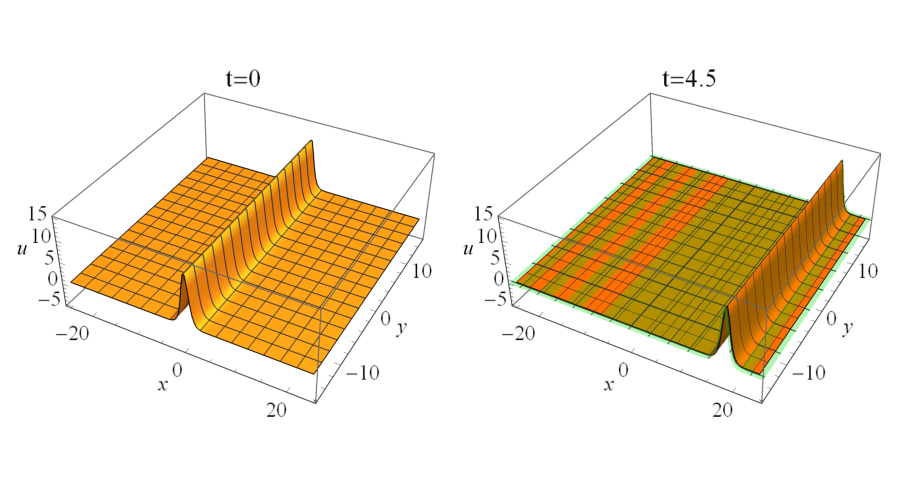
\includegraphics[width=1.0\textwidth]{figex2}
	%\caption{Stable plane wave propagation. The shape and position of the plane wave  solution at $t=4.5$ do correspond for the numerical solution (orange colored) and the analytical one (green colored).}\label{figex2}
	\caption{Устойчивое распространение плоской волны. Форма и положение решения плоской волны при $ t = 4.5 $ действительно соответствуют численному решению (оранжевый цвет) и аналитическому решению (зеленый цвет).}\label{figex2}	
\end{figure}

%Perturbed plane solitary wave soliton is studied using the initial condition developed on the basis of the asymptotic analysis (\ref{stlong}),
Устойчивость солитона в виде плоской уединенной волны исследуется с использованием начального условия, разработанного на основе асимптотического анализа (\ref {stlong}),
\begin{equation}
	\label{kp1ex2}
	u(x,y,0)=12{\text{sech}}^2(x-4t) - 2.4 {\text{cos}} (y) {\text{tanh}} (x) ~{\text{sech}}^2(x),
\end{equation}
%where $f = \pm 3$ is used in Eq. (\ref{kp3gen}).  According to the analytical solution $f=3$ corresponds to the stable case, while $f=-3$ relates to a transverse instability.
где $ f = \pm 3 $ используется в уравнении (\ref {kp3gen}). Согласно аналитическому решению, $ f = 3 $ соответствует устойчивому случаю, а $ f = -3 $ --- поперечной неустойчивости.
\begin{figure}
	\centering
	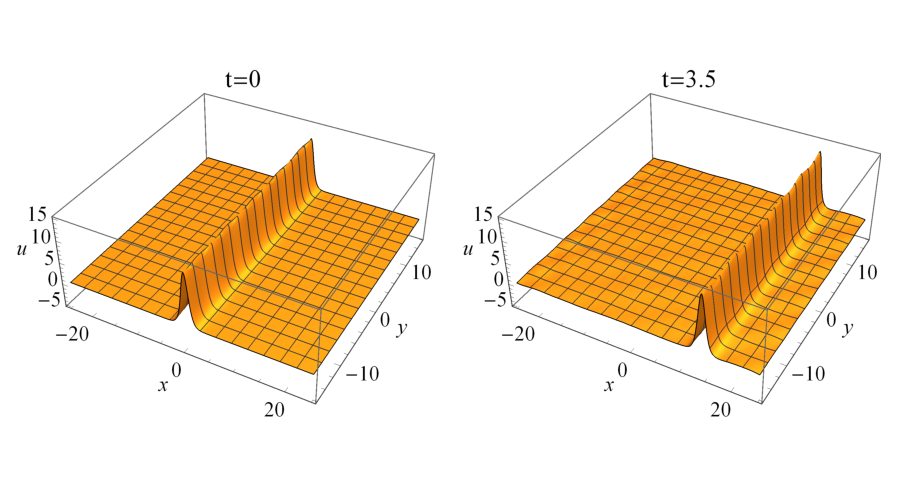
\includegraphics[width=1.0\textwidth]{fig_kp1_stable}
	%\caption{Numerical solution for the initial condition $u(x,y,0)$ for $f=3$.}\label{figex3}
	\caption{Численное решение в случае начального условия $u(x,y,0)$ при $f=3$.}\label{figex3}	
\end{figure}
\begin{figure}
	\centering
	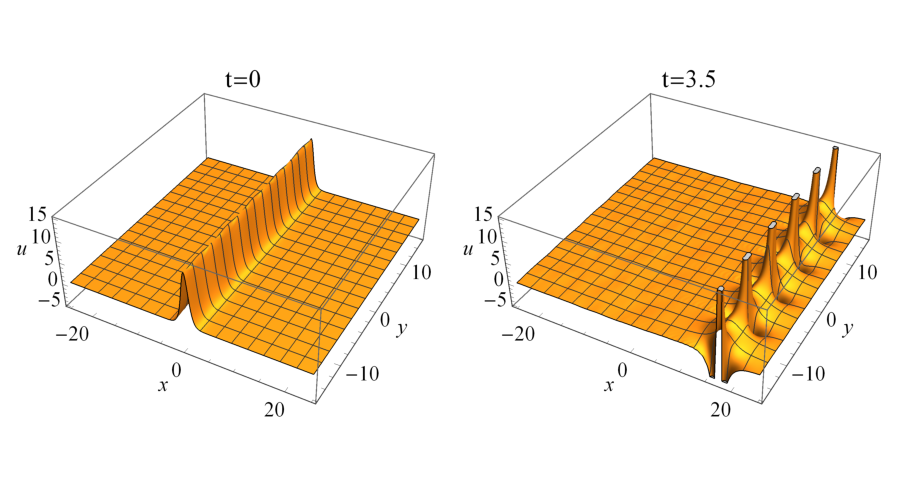
\includegraphics[width=1.0\textwidth]{fig_kp1_frw}
	%\caption{Numerical solution for the initial condition $u(x,y,0)$ for $f=-3$. The interpolation surface of the solution is cut off at $z=15$ in order to save the scale.}\label{figex4}
	\caption{Численное решение в случае начального условия $u(x,y,0)$ при $f=-3$. Поверхность интерполяции решения обрезается на $ z = 15 $ для сохранения масштаба.}\label{figex4}	
\end{figure}
\begin{figure}
	\centering
	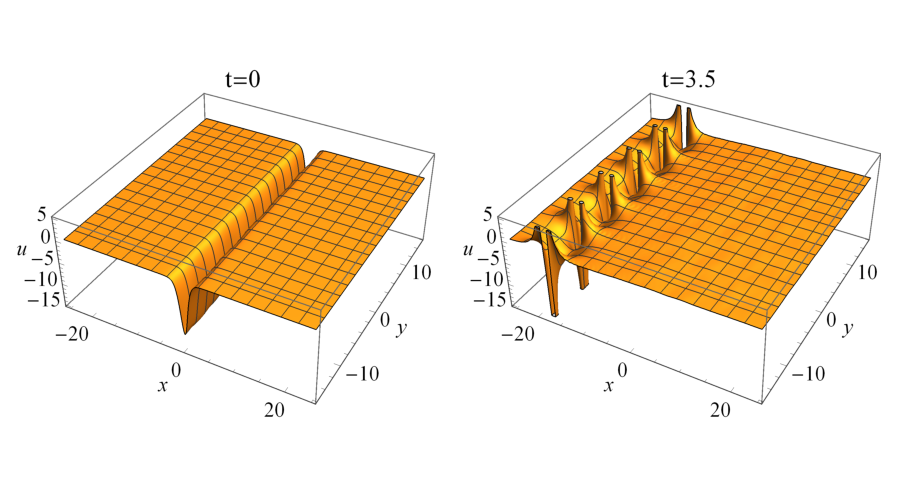
\includegraphics[width=1.0\textwidth]{fig_kp1_inverse}
	%\caption{Numerical solution for the initial condition $-u(x,y,0)$ for $f=3, c_1=-1$. The interpolation surface of the solution is cutted off at $z=-15$ in order to save the scale.}\label{figex44}
	\caption{Численное решение в случае начального условия $-u(x,y,0)$ при $f=-3, c_1=-1$. Поверхность интерполяции решения обрезается на $ z = -15 $ для сохранения масштаба.}\label{figex44}	
\end{figure}

%Comparing Figs.~\ref{figex2},~\ref{figex3} one can see the stable propagation of the plane wave in Fig.~\ref{figex3}  at the initially transversely perturbed plane wave. The wave in both figures propagates keeping its shape and velocity while initial perturbation at the wave in Fig.~\ref{figex3}  dispapear in time.
Сравнивая рис. ~ \ref{figex2}, ~\ref{figex3}, можно увидеть, что в первом случае наблюдается устойчивое распространение плоской волны на рис. ~\ref{figex3}, как и предсказывает теория. В обоих случаях волна распространяется сохраняя свою форму и скорость, при этом в первом случае возмущения исчезают со временем, а во втором --- растут.

%On the contrary, one can see in  Fig.~\ref{figex4} that the initial condition with negative $f$ provides serious transverse variations on the plane wave front. Initial small periodic perturbations suffer an increase in the amplitude and initially almost plane wave evolves into a transversely modulated wave. This happens in an agreement with an analysis. It was noted before that $c_1$ may be negative rather than $f$. However, transformation of variables, $t=-\tau$, $u=-v$, at negative $c_1$ and positive $f$ results in the obtaining equation for $v$ with positive $c_1$ and negative $f$ corresponding to an unstable propagation of negative amplitude wave $u$  (see Fig. ~\ref{figex44}).
Напротив, на рис. ~ \ref{figex4} видно, что начальное условие с отрицательным значением $ f $ приводит к серьезным поперечным изменениям на фронте плоской волны. Начальные малые периодические возмущения претерпевают увеличение амплитуды, и первоначально почти плоская волна превращается в поперечно-модулированную волну. Этот факт находится в соответствии с результатами теоретического анализа. Ранее отмечалось, что $ c_1 $ может быть отрицательным, а $ f $ --- нет. Однако преобразование переменных $ t = - \tau $, $ u = -v $ при отрицательном $ c_1 $ и положительном $ f $ приводит к получению уравнения для $ v $ с положительным $ c_1 $ и отрицательным $ f $, что соответствует неустойчивому распространению волны отрицательной амплитуды $ u $ (см. рис. ~ \ref{figex44}).

%\subsubsection{Numerical results for shear waves equation}
\subsubsection{Численные результаты для уравнения поперечных волн}

%Consider Eq.~(\ref{fkpscheme}) for $p=2$ and $\gamma \ne 0$.   
%For all simulations $N_x = 1025, N_y = 129$, time step $\Delta t = 0.003$ with 2 iterations per step. $N_x$ is chosen to be higher than it was for previous simulations in order to increase the accuracy of evaluation of the term given by Eq.~(\ref{termRY}).
Рассмотрим уравнение ~ (\ref{fkpscheme}) в случае $ p = 2 $ и $ \ gamma \ ne 0 $.
Для всех расчетов $ N_x = 1025, N_y = 129 $, временной шаг выбран равным $ \ Delta t = 0,003 $ с 2 итерациями на шаг. $ N_x $ выбрано больше, чем было для предыдущих симуляций, чтобы повысить точность оценки члена, задаваемого уравнением ~ (\ref{termRY}).

%The parameters  (\ref{solshearpar}) of exact solution (\ref{solshear}) depend on $m$ responsible for propagation inclined to the $x$ axis and two sets of parameters are possible. Therefore it is of interest to study inclined propagation of shear waves. For this purpose the initial condition is constructed as the sums of three plane wave solitons (\ref{solshear}) (at $t=0$). The distance between them is chosen  larger than their effective length, so the interaction between these solitons is very small. Also the choice of the distance provides periodic conditions for $y$ as it is seen in  Fig.~\ref{figex1025l}.
Параметры (\ref{solshearpar}) точного решения (\ref{solshear}) зависят от $ m $, ответственного за направление распространения волны относительно оси $ x $. При $m \ne 0$ необходимо сохранить условие на периодичность по обеим осям в силу ограничений численной модели. Для этого начальное условие можно построить как сумму трех солитонов плоских волн (\ref{solshear}) (при $ t = 0 $) таким образом, что периодичность сохраняется в обоих направлениях. Очевидно, что такая суперпозиция не является точным решением уравнения. Однако расстояние между солитонами выбрано больше их эффективной длины, поэтому взаимодействие между этими солитонами очень мало, и какое-то достаточно большое время плоские уединенные волны должны продолжать устойчиво распространяться с постоянной скоростью. Также выбор этого расстояния фактически обязывает изменить границы области, чтобы обеспечить периодичность, как это видно на рис. ~ \ref{figex1025l},
%The calculation domain in $x$ is increased in order to avoid the boundary influence. 
$$
L_x = 30 \pi.
$$

\begin{figure}
	\centering
	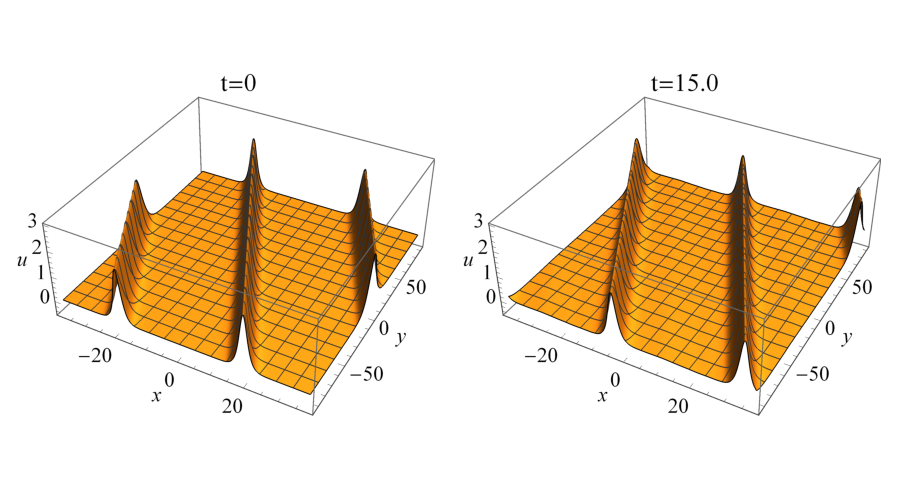
\includegraphics[width=1.0\textwidth]{figex1025l}
	%\caption{Stable inclined plane shear wave propagation. The numerical solution corresponds to the sum of three analytical plane wave  soliton solutions of Eq.~(\ref{kp3gen}) at $t = 15$.} \label{figex1025l}
	\caption{Распространение устойчивой наклонной плоской поперечной волны. Численное решение соответствует сумме трех аналитических солитонных решений плоской волны уравнения .~(\ref{kp3gen}) при $t = 15$.} \label{figex1025l}	
\end{figure}

%The initial condition is
Соответствующее начальное условие,

\begin{equation}
	\label{kp3ex2}
	u(x,y,0) = u_{\text{exact}}~(\xi ) + u_{\text{exact}}~(\xi - 2 L_y \tan \phi) + u_{\text{exact}}~(\xi + 2 L_y \tan \phi),
\end{equation}
%where
где
\begin{equation}
	u_{\text{exact}}~(\xi ) = \frac{A}{\left(Q+{\text{cosh}} (\xi )\right)},
\end{equation}
\[
A=\frac{6 c_1}{\sqrt{6 c_1 c_2+\gamma ^2 m^2}},~Q=\pm \frac{\gamma  m}{\sqrt{6 c_1 c_2+\gamma ^2 m^2}},
\]
\[
\xi = x + m y - V t, \quad V = c_1+f  m^2, \quad m = \tan{\phi}, \quad \phi = 0.2;
\]
\[
c_1 = 1, \quad c_2 = 1, \quad f = 3, \quad \gamma = 2.
\]

%The  results of stable propagation of the inclined plane waves are shown in Fig.~\ref{figex1025l}. One can check that each of inclined solitary wave corresponds to the single wave exact solitary wave solution.
Результаты устойчивого распространения наклонных плоских волн показаны на рис. ~ \ref{figex1025l}. Качественная оценка полученных результатов соответствует ожиданиям. Таким образом, численная схема позволяет оценивать свойства распространения волн в обоих направлениях и может использоваться для изучения поперечной неустойчивости плоских волн, в том числе асимметричных свойств распространения возмущений.

%To study the transverse instability we consider propagation of a single solitary wave along the $x$ axis. The perturbed initial condition is chosen according to the instability analysis of shear waves,
Для исследования поперечной неустойчивости рассматривается распространение одиночной уединенной волны вдоль оси $ x $. Возмущенное начальное условие выбирается следующим образом,
\begin{equation}
	u(x,y,0) = \sqrt{6} ~{\text{sech}}(x)-\sqrt{6}{\text{tanh}} (x) ~{\text{sech}}(x) {\text{cos}} (y),
\end{equation}
%The results are shown in Figs.~\ref{fig_good1},~\ref{fig_good3},~\ref{fig_good2}. 
Результаты расчетов продемонстрированы на рисунках .~\ref{fig_good1},~\ref{fig_good3},~\ref{fig_good2}. 
%The stable case is shown in Fig.~\ref{fig_good1} corresponds to stable case. 
%The stable case is shown in Fig.~\ref{fig_good1}.
Стабильный случай соответствует рисунку .~\ref{fig_good1}.
%One can see that the initial perturbations on the front of the wave decrease while a two-dimensionally periodic tail develops behind the plane strain  solitary wave.
Видно, что начальные возмущения на фронте волны уменьшаются, а за уединенной волной плоской деформации возникает двухмерные периодические возмущения.

\begin{figure}
	\centering
	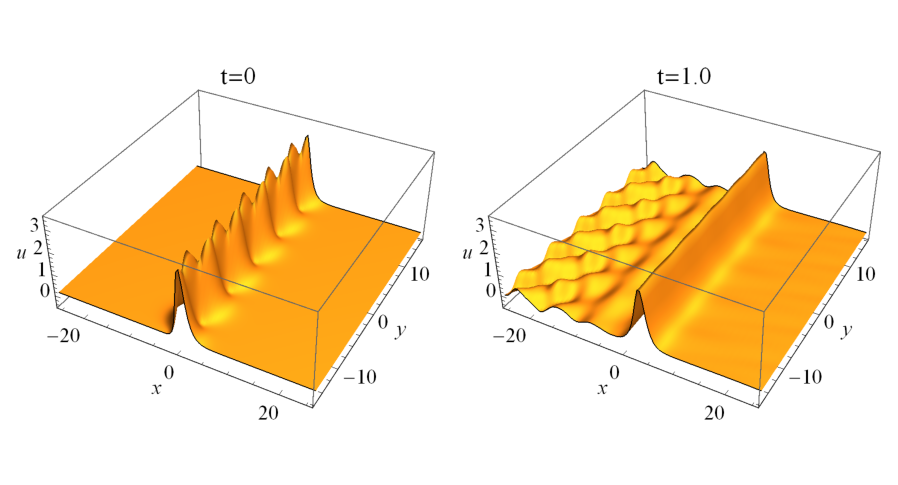
\includegraphics[width=1.0\textwidth]{fig_good1}
	%\caption{Propagation of $u(x,y,0)$ for $f = 3, \gamma = 2$} \label{fig_good1}
	\caption{Начальное условие $u(x,y,0)$ при $f = 3, \gamma = 2$} \label{fig_good1}
\end{figure}

\begin{figure}
	\centering
	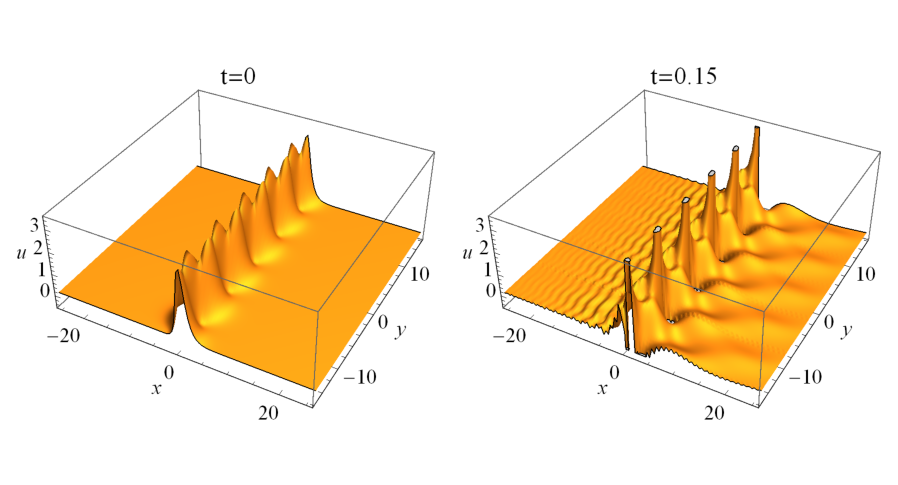
\includegraphics[width=1.0\textwidth]{fig_good3}
	%\caption{Propagation of $u(x,y,0)$ for $f = -3, \gamma = 1$} \label{fig_good3}
	\caption{Начальное условие $u(x,y,0)$ при $f = -3, \gamma = 1$} \label{fig_good3}	
\end{figure}

\begin{figure}
	\centering
	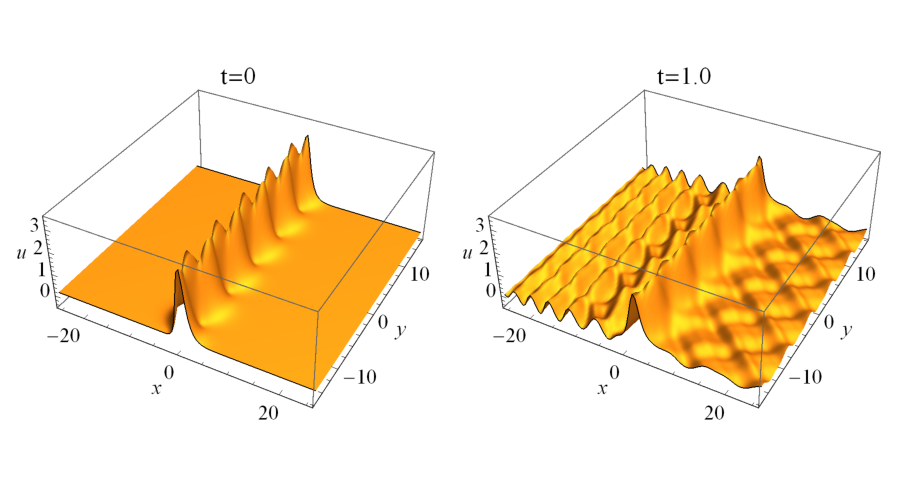
\includegraphics[width=1.0\textwidth]{fig_good2}
	%\caption{Propagation of $u(x,y,0)$ for $f = -3, \gamma = 2$} \label{fig_good2}
	\caption{Начальное условие $u(x,y,0)$ при $f = -3, \gamma = 2$} \label{fig_good2}
\end{figure}

%The unstable plane shear wave propagation is shown in  Figs.~\ref{fig_good3}, \ref{fig_good2}. In the former Figure one can see an evolution similar to that found for longitudinal waves: increase in the amplitude and deep transverse modulation of the plane wave front. The latter Figure demonstrates an influence of the value of  $\gamma $ on the transverse instability. The oscillations on the front don't grow anymore while perturbations are developing both before and after the plane wave front.
Распространение неустойчивой плоской поперечной волны показано на рис. ~ \ref {fig_good3}, \ref{fig_good2}. На первом рисунке можно увидеть эволюцию, аналогичную той, что наблюдается для продольных волн: увеличение амплитуды и глубокая поперечная модуляция фронта плоской волны. Последний рисунок демонстрирует влияние значения $ \gamma $ на поперечную неустойчивость. Колебания на фронте больше не нарастают, а возмущения развиваются как до, так и после фронта плоской волны.

\fixme{Далее ожидается добавить более корректное обобщение численной схемы, так как текущая не является полноценной и была сделана лишь для получения результатов <<любым>> способом. В таком случае ее можно будет представить к защите.}


\subsection{Другие численные решения}
\textbf{Equation for shear strains and its solution}

The governing equation for shear waves reads \cite{PorKrOs, poosan20}
\begin{equation}
	v_{xt} +c_1~F_{xxxx}+ c_2~ v_{x}^2~ v_{xx}+\lambda v_{yy}+\gamma~v_{y}~ v_{xx}~=~0, \label{kpsh}
\end{equation}
where $v(x,t)$ is a shear displacement, $c_i$, $\lambda$, $\gamma$ are the constants. 

One can see that Eq. (\ref{kpsh}) is not invariant under the transformation $y\rightarrow -y$.  Consider its plane traveling wave solution depending only on the phase variable $\xi=x+ m y-V t$ and assume that $u=v_x$. 
The solution, obtained by using direct integration, reads
\begin{equation}
	u=\frac{A}{Q+{\text{cosh}}( \beta \xi)},\label{solshear}
\end{equation}
where
\begin{equation}
	A=\pm \frac{6c_1 \beta^2}{\sqrt{\gamma^2 m^2+6 c_1 c_2 \beta^2}}, 
	Q_{\pm}=\pm\frac{\gamma m }{\sqrt{\gamma^2 m^2+6 c_1 c_2 \beta^2}},  V=\beta^2 c_1+m^2 \lambda . \label{solshearpar}
\end{equation}
We consider only bounded solutions when $Q<1$. This is guaranteed if $c_1 c_2>0$, and the solutions with both $Q_{+}$  and $Q_{-}$ being bounded. Otherwise only positive $Q_{\pm}$ give rise to a bounded solution.  The sign of $Q$ depends on the sign of the parameter $m$ responsible for the angle of the wave front propagation relative to the $x$- axis and the sign of the denominator.  However, the presence of $\pm$ in the expression for $Q_{\pm}$ discards the dependence on the sign of $m$. The sign of the amplitude $A/(Q+1)$ of the bounded solution is not sensitive to the sign of $m$. 
\begin{figure}[h]
	\begin{center}
		\begin{tabular}{cc}
			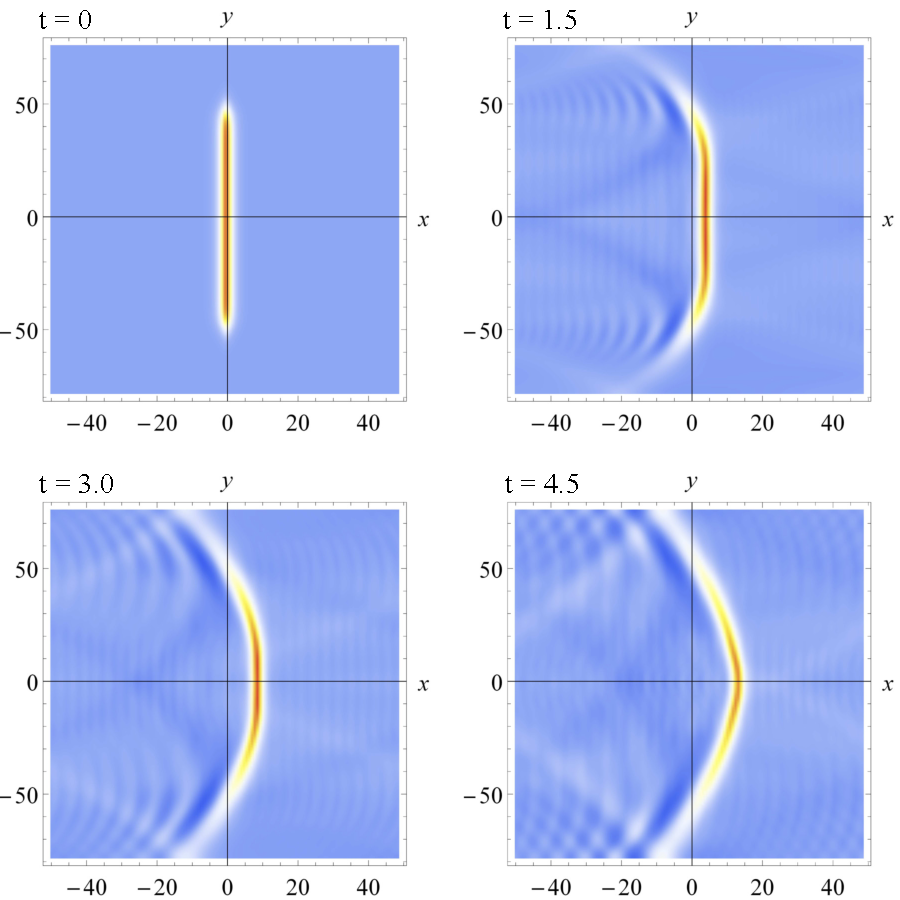
\includegraphics[scale=0.7]{fig1t.pdf} & 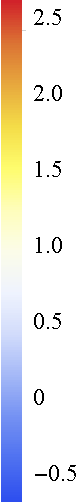
\includegraphics[scale=0.6]{palette.pdf}
		\end{tabular}
		\caption{Evolution of the shear strain wave(\ref{init}) in Case 1.}\label{fig1}
	\end{center}
\end{figure}
For the wave propagating along $x$ axis we have $m=0$ and $Q=0$. Then the familiar solitary wave solution to the modified Korteweg-de Vries equation appears from (\ref{solshear}),
\begin{equation}
	q_m=\pm \frac{6c_1\beta}{\sqrt{6 c_1 c_2}}{\text{cosh}}^{-1}(\beta \xi) \label{qp}
\end{equation}
that exists only when $c_1 c_2>0$. 

\section{Numerical study of nonlinear shear strains localization}
Let us re-write Eq. (\ref{kpsh}) through the shear strain, 
\begin{equation}
	\label{kp3gen}
	\partial_x\left(\partial_t u+c_1 \partial_{xxx} u+\frac{c_2 }{3}\partial_x u^{3}\right)+\lambda \partial_{yy} u+\gamma \partial_x\left(\partial_x u \int_{-\infty}^x \partial_y u \, dx'\right)=0.
\end{equation}
\begin{figure}
	\begin{center}
		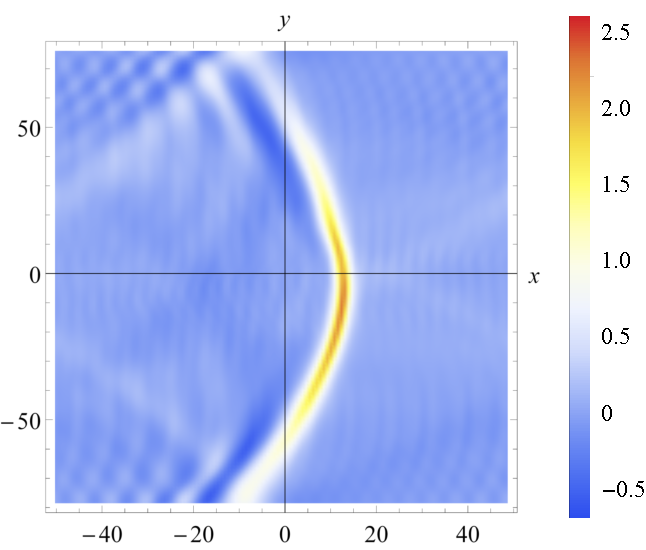
\includegraphics[scale=0.7]{fig2_instead.pdf} 
		\caption{Transformation to an asymmetric profile in Case 2 at t = 4.5.}\label{fig2}
	\end{center}
\end{figure}
\begin{figure}
	\begin{center}
		\begin{tabular}{cc}
			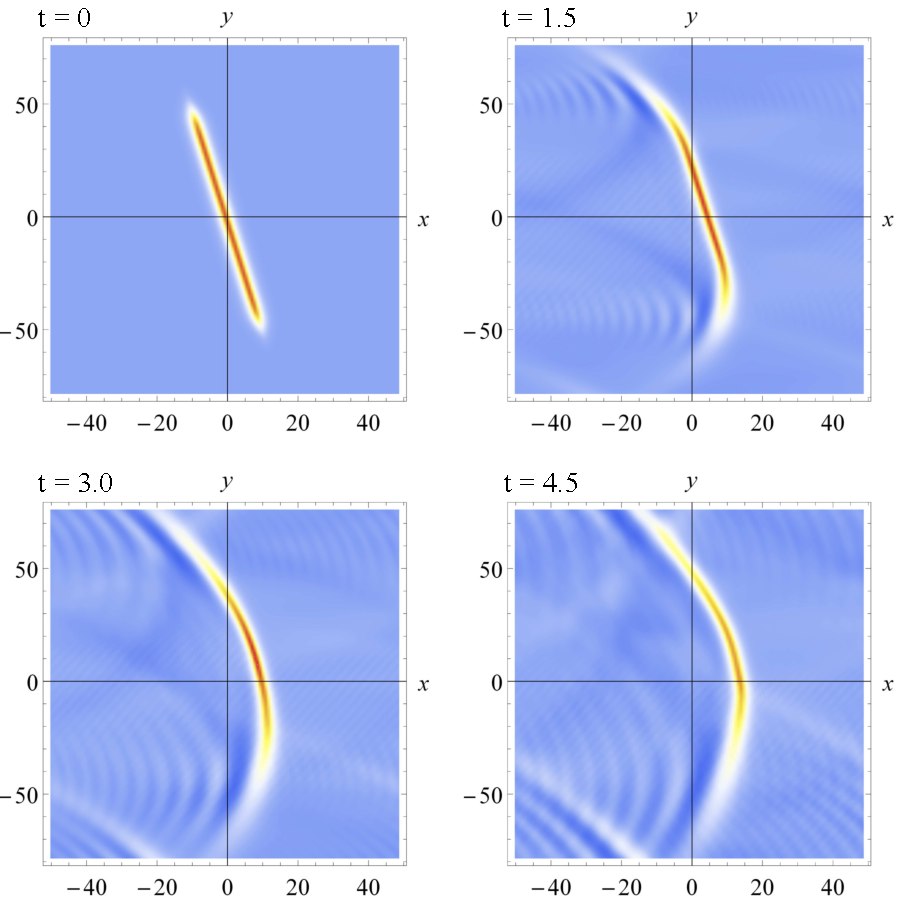
\includegraphics[scale=0.6]{fig3t.pdf} & 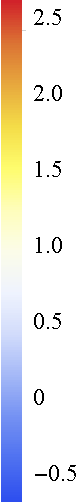
\includegraphics[scale=0.6]{palette.pdf}
		\end{tabular}
		\caption{Asymmetry for the initial condition corresponding to Case 3.}\label{fig3}
	\end{center}
\end{figure}
The Fourier spectral method is used here to solve Eq.~(\ref{kp3gen}) numerically. More detailed information about the method can be found in \cite{poosan20}.
In all the simulations we put $c_1 = 1$, $c_2 = 1$ and $\lambda = 3$. The initial condition is assumed as
\begin{equation}\label{init}
	u_0 = \frac{\sqrt{6}\;\mathrm{sech}(X)}{10^{-8} \mathrm
		{cosh} (0.6 Y)+1}.
\end{equation}
The values of $X, Y$ and $\gamma$ are varied as shown in Table~\ref{table1}.

\begin{figure}
	\begin{center}
		\begin{tabular}{cc}
			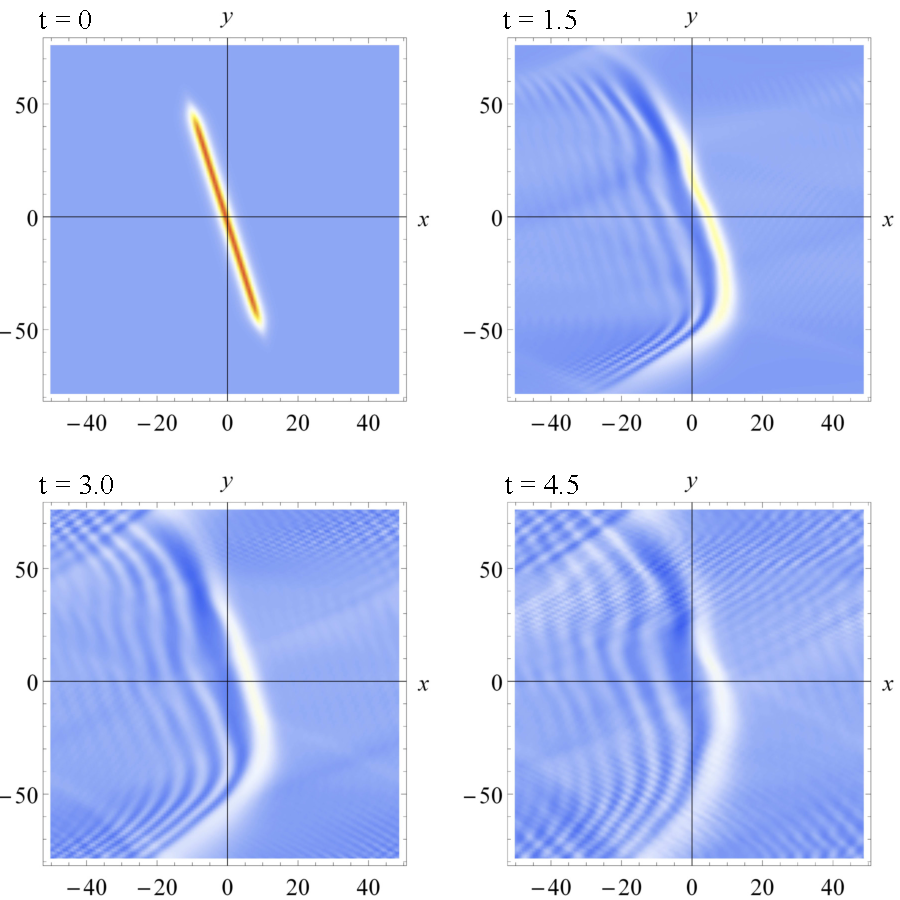
\includegraphics[scale=0.6]{fig4t.pdf} & 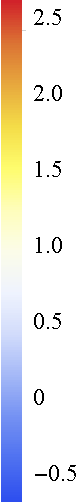
\includegraphics[scale=0.6]{palette.pdf}
		\end{tabular}
		\caption{Scattering of the initial condition corresponding to Case 4.}\label{fig4}
	\end{center}
\end{figure}
\begin{table}[h!]
	\centering
	\begin{tabular}{|l|l|l|l|}
		\hline
		& $X$ & $Y$ & $\gamma$\\ \hline
		Case 1 &  $x$   & $y$  & 0 \\ \hline
		Case 2 &   $x$   &   $y$ & 1 \\ \hline
		Case 3 &  $x \cos (0.2 )+y \sin (0.2 )$   &   $x \cos (0.2 )+y \sin (0.2 )$ & 1\\ \hline
		Case 4 &   $x \cos (0.2 )+y \sin (0.2 )$  &  $x \cos (0.2 )+y \sin (0.2 )$  & 5\\ \hline
	\end{tabular}
	\caption{Expressions of $X, Y$ for the initial conditions.}\label{table1}
\end{table}


\textbf{Case 1}. In Fig.~\ref{fig1} the symmetric relative to the $x$-axis propagation of the strain wave (\ref{init}) is shown. The curvature of the wave profile develops in time and a scattering of the wave happens behind the curved wave front. The amplitude and the velocity of the wave  decrease in  time. 

\textbf{Case 2}. The initial profile suffers from asymmetric variations relatively to the $x$-axis, see Fig. \ref{fig2}. The highest  amplitude is not reached on the $Ox$ axis. However, changing the sign of $\gamma$ does not provide additional non-symmetry.   

\textbf{Case 3}. The role of quadratic nonlinearity on the initially inclined wave is shown in Fig. \ref{fig3}. It is quite similar to what is shown in Fig.~\ref{fig2}. The presence of the nonlinear term changes the direction of wave propagation in the similar way as in Case 2. The amplitude and velocity  also decrease in time.

\textbf{Case 4}. One can see in Fig. \ref{fig4} that an increase in the value of $\gamma$ results in a  scattering behind the wave front.

%\section{Conclusions}
\section{Заключение}

\fixme{Переделать}

%The asymptotic technique presented in this paper allows to reduce the coupled nonlinear continuum equations of 2D crystal lattices to a single nonlinear equation for strain waves, which allows to analyze only relevant terms in the new equations.
%Two types of lattices were considered: the generalized square lattice and the graphene lattice (the model is based on a consideration of two interacting sub-lattices with both translational and angular interactions being taken into account), and the governing two-dimenisonal equations for longitudinal and shear strain waves. Their exact plane wave solutions and their transverse stability have been revealed  in  numerical simulations.

%Numerical simulations confirm  that the angular stiffness in the original discrete model gives rise to various types of nonlinear waves localization depending on the coefficients values. Previous studies of the lattices of another structure revealed important variations in the governing equation from that of the longitudinal waves \cite{porkros}.
%Extended interactions in the square lattice firstly produce additional extrema in the dispersion curve for linear longitudinal plane waves. They have a significant influence on the auxetic behavior of the material. One can note that the one-dimensional limits of the equations for longitudinal and shear waves differ only by nonlinear terms (quadratic or cubic) while two-dimensional consideration results in different transverse variation terms which are nonlinear for shear waves contrary to the linear term for longitudinal waves. Moreover, the sign of the coefficients in the governing equations may vary more for shear waves descriptions. It results in different stability criteria for longitudinal and shear localized plane strain waves. 

%This, in turns it allows us to predict different scenario of the wave amplification and localization due toa  transverse instability caused by the values of the coefficients of rigidity. In the stable case of the Kadomtsev-Petviashvili equation (\ref{kp}) two-dimensional localized wave amplification happens due to instability, see Figs. \ref{figex4}, \ref{figex44}. An unstable case of Eq. (\ref{kp}) also results in the transverse periodic modulation of the plane wave. Figure  \ref{figex4} demonstrated classical result for the corresponding negative sign at the term with derivatives with respect to $y$. However, this case is not realized for description of our lattice while the negative sign at the dispersion term can be achieved. This results in the dynamics shown in Fig.  \ref{figex44}. The new results concern the transverse instability of nonlinear shear waves, see Figs. ~\ref{fig_good3}, \ref{fig_good2} which is different from that of longitudinal waves.
%The comparison of the numerical results for shear waves gives an explanation, how the coefficient at the quadratic nonlinearity influences the inclined plane solitary wave  propagation and the transverse instability.  

%One of the potential extensions of this study is a  short-range wave continualization. Previously it was studied for a hexagonal lattice in Refs. \cite{PorBer, PorBer2} where new model modulation two-dimensional equations were obtained. Also, nonlocal interactions will be of interest, in particular, utilization of the method of using shift operators \cite{Mich} for obtaining two-dimensional model equations for dynamical processes in nonlocal square lattice will be considered in the nearest future.
%Another extension of the model concerns an inclusion of the geometrical nonlinearity in the discrete model like it was done, e.g., in (\cite{karima}).
%Furthermore, along with the geometrical nonlinearity and weakly transversely perturbed shear waves, the study can be extended to the case of nonlinear translational stiffnesses examination.

%Асимптотическая техника, представленная в этой статье, позволяет свести связанные нелинейные уравнения континуума двумерных кристаллических решеток к одному нелинейному уравнению для волн деформации, что позволяет анализировать только соответствующие члены в новых уравнениях.
\fixme{Были рассмотрены два типа решеток: обобщенная квадратная решетка и решетка графена (модель основана на рассмотрении двух взаимодействующих подрешеток с учетом как поступательного, так и углового взаимодействия) и определяющие двумерные уравнения для продольных и волны сдвига деформации}. Их точные решения в виде плоских волн и их поперечная устойчивость были выявлены в ходе численного моделирования.

Численное моделирование подтверждает, что угловая жесткость в исходной дискретной модели приводит к различным типам локализации нелинейных волн в зависимости от значений коэффициентов. Предыдущие исследования решеток другой структуры выявили важные отличия основного уравнения от уравнения продольных волн \cite {porkros}.
Расширенные взаимодействия в квадратной решетке сначала создают дополнительные экстремумы на дисперсионной кривой для линейных продольных плоских волн. Они оказывают значительное влияние на ауксетическое поведение материала. Можно отметить, что одномерные пределы уравнений для продольных и поперечных волн отличаются только нелинейными членами (квадратичными или кубическими), в то время как двумерное рассмотрение приводит к различным членам поперечной вариации, которые являются нелинейными для поперечных волн в отличие от линейного члена для продольные волны. Более того, знак коэффициентов в определяющих уравнениях может больше различаться для описания поперечных волн. Это приводит к различным критериям устойчивости продольных и сдвиговых локализованных волн плоской деформации.

Это, в свою очередь, позволяет прогнозировать различные сценарии усиления и локализации волн из-за поперечной неустойчивости, вызванной значениями коэффициентов жесткости. В устойчивом случае уравнения Кадомцева-Петвиашвили (\ref {kp}) двумерное локализованное усиление волн происходит из-за неустойчивости, см. Рис. \ref {figex4}, \ref {figex44}. Неустойчивый случай уравнения (\ref {kp}) также приводит к поперечной периодической модуляции плоской волны. На рисунке \ref {figex4} показан классический результат для соответствующего отрицательного знака у члена с производными по $ y $. Однако этот случай не реализуется для описания нашей решетки, а отрицательный знак у дисперсионного члена может быть достигнут. Это приводит к динамике, показанной на рис. \ref{figex44}. Новые результаты касаются поперечной неустойчивости нелинейных поперечных волн, см. Рис. ~ \ref {fig_good3}, \ref{fig_good2}, который отличается от продольных волн. Сравнение численных результатов для поперечных волн дает объяснение, как коэффициент при квадратичной нелинейности влияет на распространение наклонной плоской уединенной волны и поперечную неустойчивость.
